% !TeX root = ../libro.tex
% !TeX encoding = utf8
\chapter{Función Distancia con Signo}
Tenemos como objetivo representar superficies en $\R^3$. En general, estas pueden estar definidas de multitud de formas, siendo una de las más usuales a través de una función implícita. Nosotros nos centraremos en un tipo especial de funciones implícitas, que introducimos a continuación.

\begin{definicion}
  Sea $\Omega \subseteq \R^3$. Una \textbf{función distancia} es aquella que a cada punto de $\R^3$ le asigna su menor distancia a la frontera de $\Omega$:
    \begin{align*}
          d_{\Omega} \colon \R^3 &\to \R_0^+.\\
          x &\mapsto \inf\{\Vert x-y\Vert) \colon y \in \delta\Omega\}.
    \end{align*}

    Cuando $\Omega$ sea cerrado, podremos usar el mínimo en lugar del ínfimo.
\end{definicion}
 
\begin{definicion}[SDF]\label{d:sdf}
  Sea $\Omega \subseteq \R^3$. Una \textbf{función distancia con signo} es una función de la forma:
  \begin{align*}
          \phi_{\Omega} \colon \R^3 &\to \R.\\
          x &\mapsto \begin{cases}
      d_{\Omega}(x),  &x\in \R^3\setminus \mathring{\Omega}. \\
      -d_{\Omega}(x), &x\in \mathring{\Omega}.
    \end{cases}
    \end{align*}

  En general, nos referiremos a esta función por sus siglas en inglés SDF (\textit{Signed Distance Function}), y la denotaremos simplemente $\phi$ siempre que no haya confusión.
\end{definicion}

\begin{definicion}
  Dada una función $\phi\colon \R^3 \to \R$ y $k\in\R$, llamamos \textbf{isosuperficie de $\boldsymbol{\phi}$ con valor $\boldsymbol{k}$} al conjunto:
  \begin{equation*}
      S_{\phi,k} = \{(x,y,z) :  \phi(x,y,z)=k\}.
  \end{equation*}
  Sin pérdida de generalidad podemos suponer $k=0$, pues de no ser el caso, tomamos la función $\phi'(x,y,z)=\phi(x,y,z)-k$ y tenemos que $S_{\phi',0} = S_{\phi,k}$. Por tanto, la denotaremos como $S_\phi$.
\end{definicion}

Nuestra intención será entonces construir una escena definida como la isosuperficie generada por un SDF. A partir de ahora, tomaremos $p=(x,y,z)\in\R^3$.

\begin{ejemplo}
    Ejemplos simples de SDF $\phi$ en $p$ para diferentes conjuntos $\Omega$ son:
    \begin{itemize}
        \item \textbf{Esfera de radio $\boldsymbol{r}$ centrada en el origen.}
        \begin{equation*}
            \Omega=\{x\in \R^3 : \Vert x\Vert = r\},\quad \phi(p) = \Vert p\Vert - r.
        \end{equation*}
        \item \textbf{Plano con vector normal unitario $\boldsymbol{n=(a,b,c)}$ y pasando por el origen}.
        \begin{equation*}
            \Omega=\{p\in\R^3 : ax+by+cz = 0\},\quad \phi(p) = p\cdot n.
        \end{equation*}
        \item \textbf{Toro de radios $\boldsymbol{R}$ y $\boldsymbol{r}$, con $\boldsymbol{R>r}$}:
        \begin{equation*}
            \Omega=\left\{p\in \R^3 : \left(R-\sqrt{x^2+y^2}\right)^2 + z^2 = r^2\right\},\quad \phi(p)= \bigg\Vert (\Vert(x,0,z)\Vert - R, y) \bigg\Vert - r.
        \end{equation*}
    \end{itemize}
\end{ejemplo}


\section{Operaciones sobre SDF}
Si bien estas primitivas son fáciles de generar, también son muy simples y nos serán insuficientes si queremos construir escenas más complejas. Una de las ventajas de los SDF es que se pueden generar nuevas formas a partir de primitivas de forma muy sencilla. Para ello, una de las técnicas más útiles es la geometría de sólidos constructiva, que utiliza operaciones booleanas para combinar múltiples primitivas. Por la naturaleza de los SDF, estas operaciones se implementan fácilmente usando las funciones $\Max$ y $\Min$.

\begin{definicion}[Operaciones Booleanas]\label{p:boolean}
    Sean $A$ y $B$ isosuperficies generadas por $\phi$ y $\gamma$ respectivamente. Definimos los SDF para las siguientes operaciones.
    \begin{itemize}
        \item \textbf{Unión: } $\sdf_{A\cup B}(p) = \Min(\phi(p), \gamma(p))$,
        \item \textbf{Intersección: } $\sdf_{A\cap B}(p) = \Max(\phi(p), \gamma(p))$,
        \item \textbf{Diferencia: } $\sdf_{A\setminus B}(p) = \Max(\phi(p), -\gamma(p))$.
    \end{itemize}
\end{definicion}

\begin{observacion}
    Solo en el caso de la unión se obtiene un SDF según lo establecido en la \autoref{d:sdf}, ya que al aplicar $\Max$ en el interior (donde $\phi < 0$), las funciones resultado pueden ser solo una cota superior de la distancia. En nuestro caso solo estamos interesados en visualizar la frontera de las superficies, así que podemos obviar este problema.
\end{observacion}

Un problema de usar estas transformaciones es que produce discontinuidades en la derivada del SDF resultante. Trataremos de evitar esta situación, además de por motivos analíticos, por motivos visuales, ya que el resultado de estas operaciones produce bordes muy acusados en la intersección de ambas superficies. Existen muchas formas de combinar SDF de forma más natural. Usaremos una de las más extendidas, usada por programas de modelado 3D como Blender \cite{repo:blender} o videojuegos como \cite{game:dreams}, y ha sido estudiada por Íñigo Quilez en su web \cite{article:smooth}.

\begin{observacion}
    Para mayor claridad, en las figuras se representarán funciones de variable real, a pesar de que en nuestro caso sería en $\R^3$.
\end{observacion}

Empezamos centrándonos en la unión. La idea es, dadas $\phi$ y $\gamma$, añadir una corrección para cada punto a la función $\Min$ original para que cumpla ciertos requisitos. Además esta función tendrá un parámetro $k\in\R$ que permita controlar su influencia. Llamaremos a esta corrección $\omega\colon \R^3\times \R^+_0\to\R$, de forma que la versión suavizada de $\Min$ será:
\begin{align*}
          \smin\colon \R^3\times \R^+_0 &\to \R.\\
          (p,k) &\mapsto \Min(\phi(p),\gamma(p)) - \omega(p,k).
    \end{align*}

Como no queremos que este cambio afecte al algoritmo de \textit{raymarching}, debe cumplirse $\Min(p)\ge \smin(p) \ \forall p \in \R^3$, esto es, $\omega(p)\ge 0\ \forall p \in \R^3$. 
Si estudiamos como se comporta la versión real de $\Min$ en la \autoref{fig:min_real}, vemos que hay que corregirla cerca de las intersecciones de $\phi$ y $\gamma$, es decir, cuando $\phi$ y $\gamma$ estén arbitrariamente cerca. En el resto de puntos no queremos modificar la función original, luego estudiamos el comportamiento de $\smin$ en la bola cerrada centrada en $p$ de radio $k$:
\begin{equation*}
    B_{p,k} = \{p\in\R^3 : |\phi(p)-\gamma(p)| \le k\}, \ p\in \R^3,\ k\in\R^+_0
\end{equation*}

siendo $\omega(p) = 0$ cuando $p\notin B_{p,k}$. 

\begin{figure}[t]
    \centering
    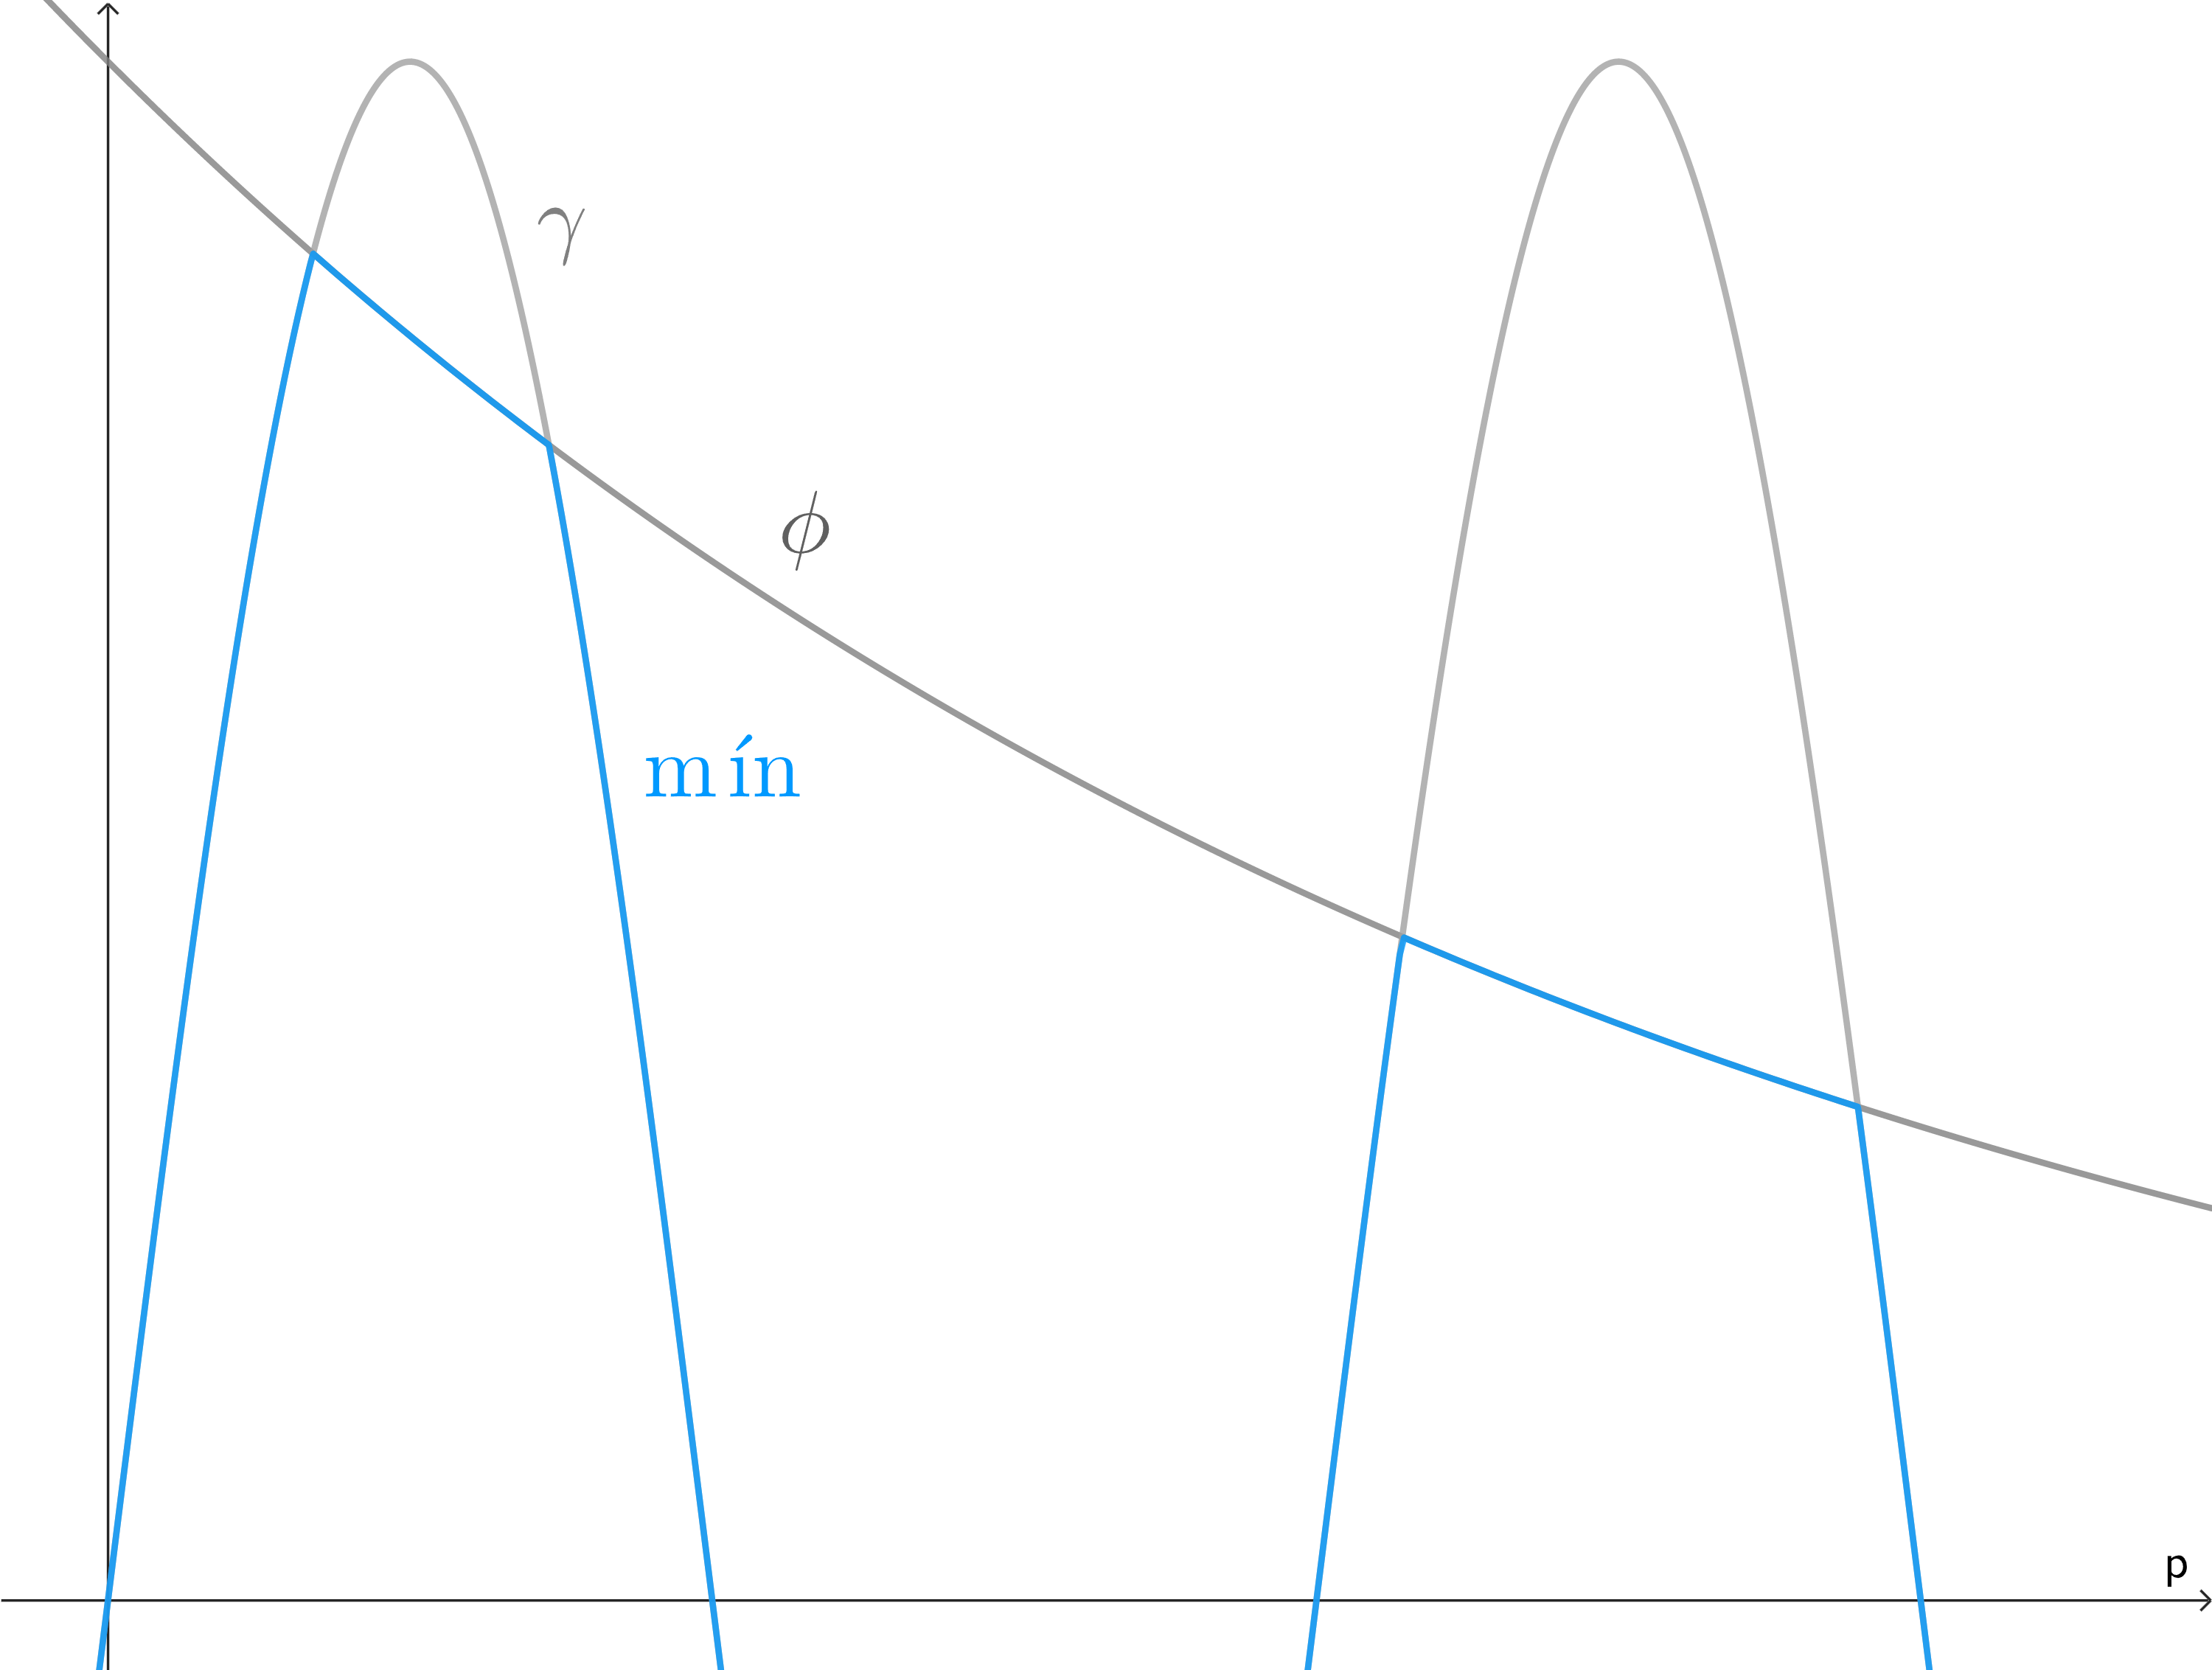
\includegraphics[width=\textwidth]{Plantilla-TFG-master/img/smooth_real.png}
    \caption{Gráfica de $\Min\colon \R\to\R$}
    \label{fig:min_real}
\end{figure}

Como queremos que $\smin$ sea continua en la frontera de $B_{p,k}$, imponemos la condición $\omega(p) = 0\ \forall p \in \delta B_{p,k}$. Por otro lado, es lógico que $\omega$ alcance su valor máximo en el punto de intersección, luego imponemos también $\omega(p) = s$, donde $s\in\R$ es el máximo de $\omega$ en $B_{p,k}$, y deberemos ajustarlo más adelante. Con estos requisitos, tenemos una primera aproximación para $\omega$ dado $p\in B_{p,k}$:
\begin{equation*}
    \omega(p,k) = s\left( 1-\frac{|\phi(p)-\gamma(p)|}{k} \right)^n = \begin{cases}
        s\left( 1-\frac{\phi(p)-\gamma(p)}{k}\right)^n,\ \phi(p)>\gamma(p) \\[10pt]
        s\left( 1+\frac{\phi(p)-\gamma(p)}{k}\right)^n,\ \phi(p)\le \gamma(p)\\[10pt]
    \end{cases}  ,\ s\in\R,\ n\in\N,
\end{equation*}
donde hemos añadido el parámetro $n$ para añadir más control al resultado final. Es evidente que está bien definida, pues:
\begin{equation*}
    \phi(p)=\gamma(p) \implies \frac{\phi(p)-\gamma(p)}{k} = 0\implies \omega(p) = s
\end{equation*}


\begin{figure}[!h]
     \begin{minipage}[c]{0.49\linewidth}
        \centering
        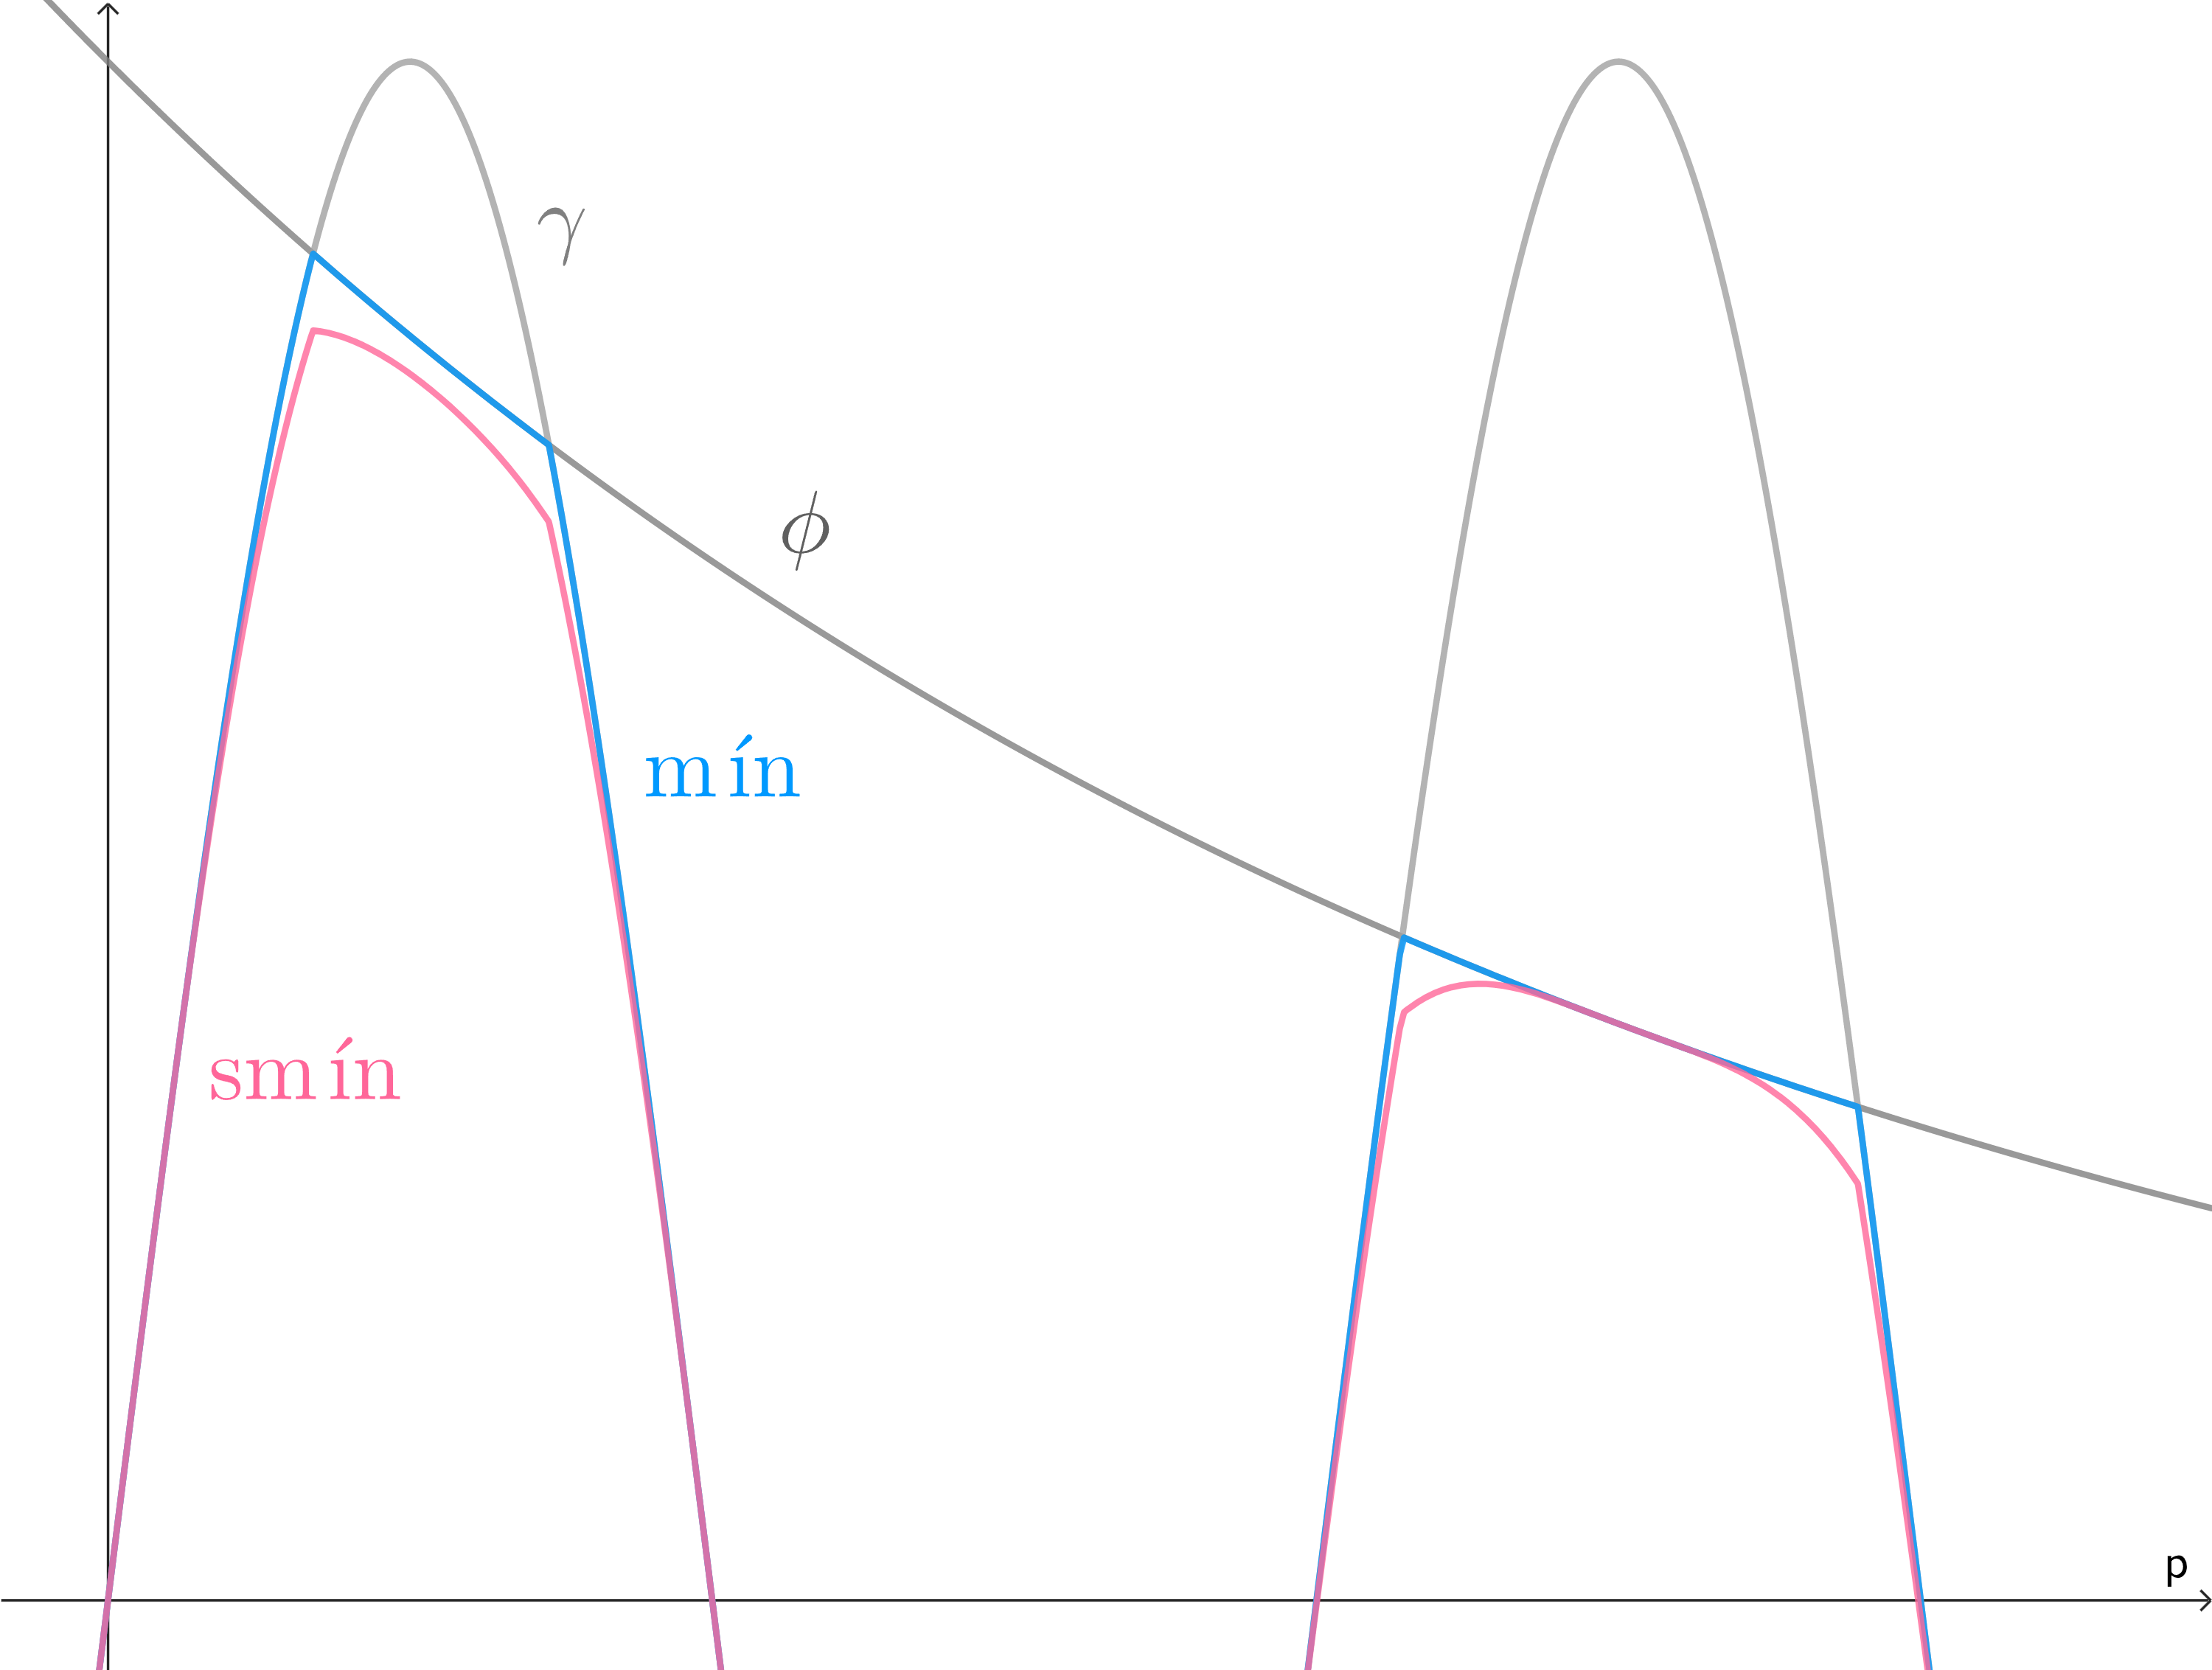
\includegraphics[width=0.95\textwidth]{Plantilla-TFG-master/img/smin_1.png}
        \caption{$k=0.6$}
     \end{minipage}
     \begin{minipage}[c]{0.49\linewidth}
        \centering
        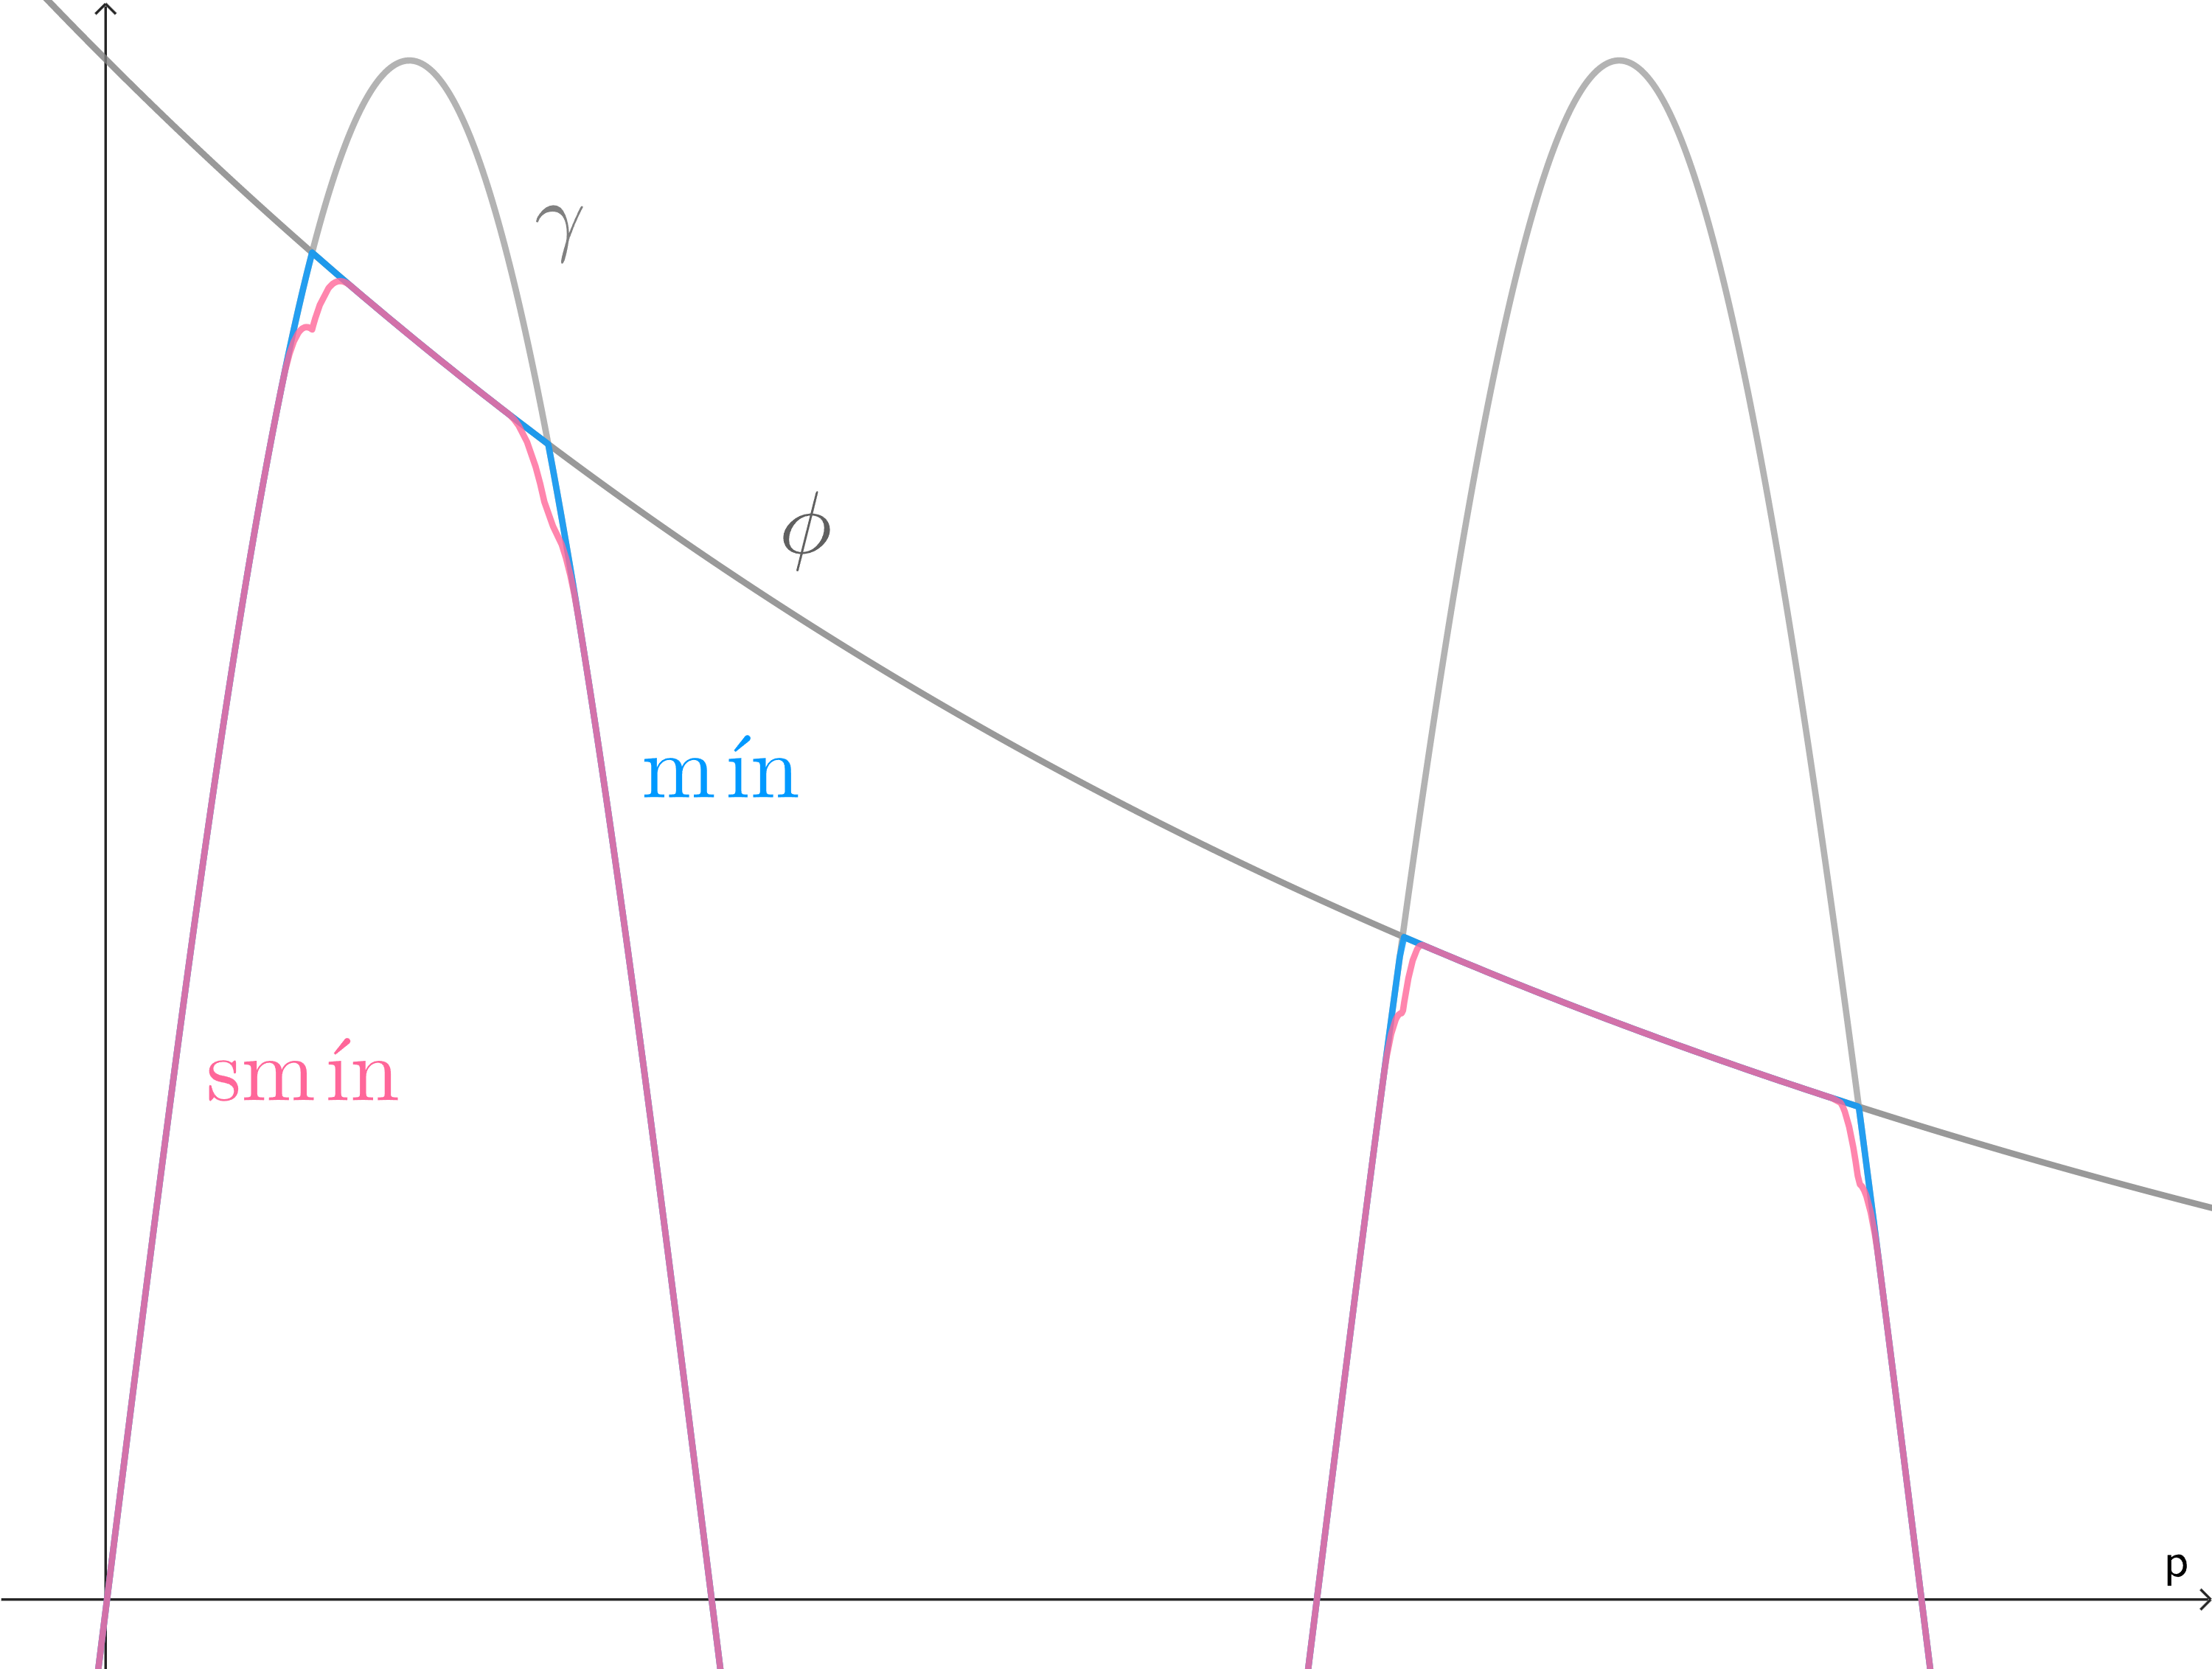
\includegraphics[width=0.95\textwidth]{Plantilla-TFG-master/img/smin_2.png}
        \caption{$k=0.1$}
     \end{minipage}
     \caption{Primera aproximación de $smin(p,k)$ con $s=0.05$ y $n=2$}
     \label{fig:smooth1}
\end{figure}

 Pasamos ahora a solucionar el problema inicial, el de la continuidad de la derivada. 
\begin{align*}
    \smin'(p,k) &=  \left(\Min(\phi(p),\gamma(p))\right)' - \omega(p,k)'\\[10pt] &= \begin{cases}
        \gamma'(p) + sn\left(1-\frac{\phi(p)-\gamma(p)}{k}\right)^{n-1}\left(\frac{\phi'(p)-\gamma'(p)}{k}\right),\ \phi(p)>\gamma(p) \\[10pt] 
        \phi'(p) - sn\left(1+\frac{\phi(p)-\gamma(p)}{k}\right)^{n-1}\left(\frac{\phi'(p)-\gamma'(p)}{k}\right),\ \phi(p)\le \gamma(p)
    \end{cases}
\end{align*}

Dado $c\in\R^3$ tal que $\phi(p) = \gamma(p)$, veamos cuando está bien definida:
\begin{align*}
    \phi' - sn\left(1+\frac{\phi-\gamma}{k}\right)^{n-1}\left(\frac{\phi'-\gamma'}{k}\right) &= \gamma' + sn\left(1-\frac{\phi-\gamma}{k}\right)^{n-1}\left(\frac{\phi'-\gamma'}{k}\right)
\end{align*}
Evaluando en $c$:
\begin{align*}
    \cancel{\phi'(c) -  \gamma'(c)} &= 2sn\left(1+\frac{\phi(c)-\gamma(c)}{k}\right)^{n-1}\left(\frac{\cancel{\phi'(c)-\gamma'(c)}}{k}\right);\\
    s &= \frac{k}{2n}\left(1-\frac{\cancelto{0}{\phi(c)-\gamma(c)}}{k}\right);\\
    s &= \frac{k}{2n}
\end{align*}
    


Hemos llegado a la expresión final
\begin{align*}
    \omega(p,k) &= \begin{cases}
        \frac{k}{2n}\left( 1-\frac{|\phi(p)-\gamma(p)|}{k} \right)^n,\ &|\phi(p)-\gamma(p)|\le k,\\[10pt]
        0,\ &\text{ otro caso }
    \end{cases}\\[10pt] &= \frac{\Max\left( k - |\phi(p) - \gamma(p)|, 0\right)^n}{2n\cdot k^{n-1}}  ,\ s\in\R,\ n\in\N,
\end{align*}

Podemos observar los resultados en la \autoref{fig:smooth2}.
\begin{figure}[!h]
     \begin{minipage}[c]{0.49\linewidth}
        \centering
        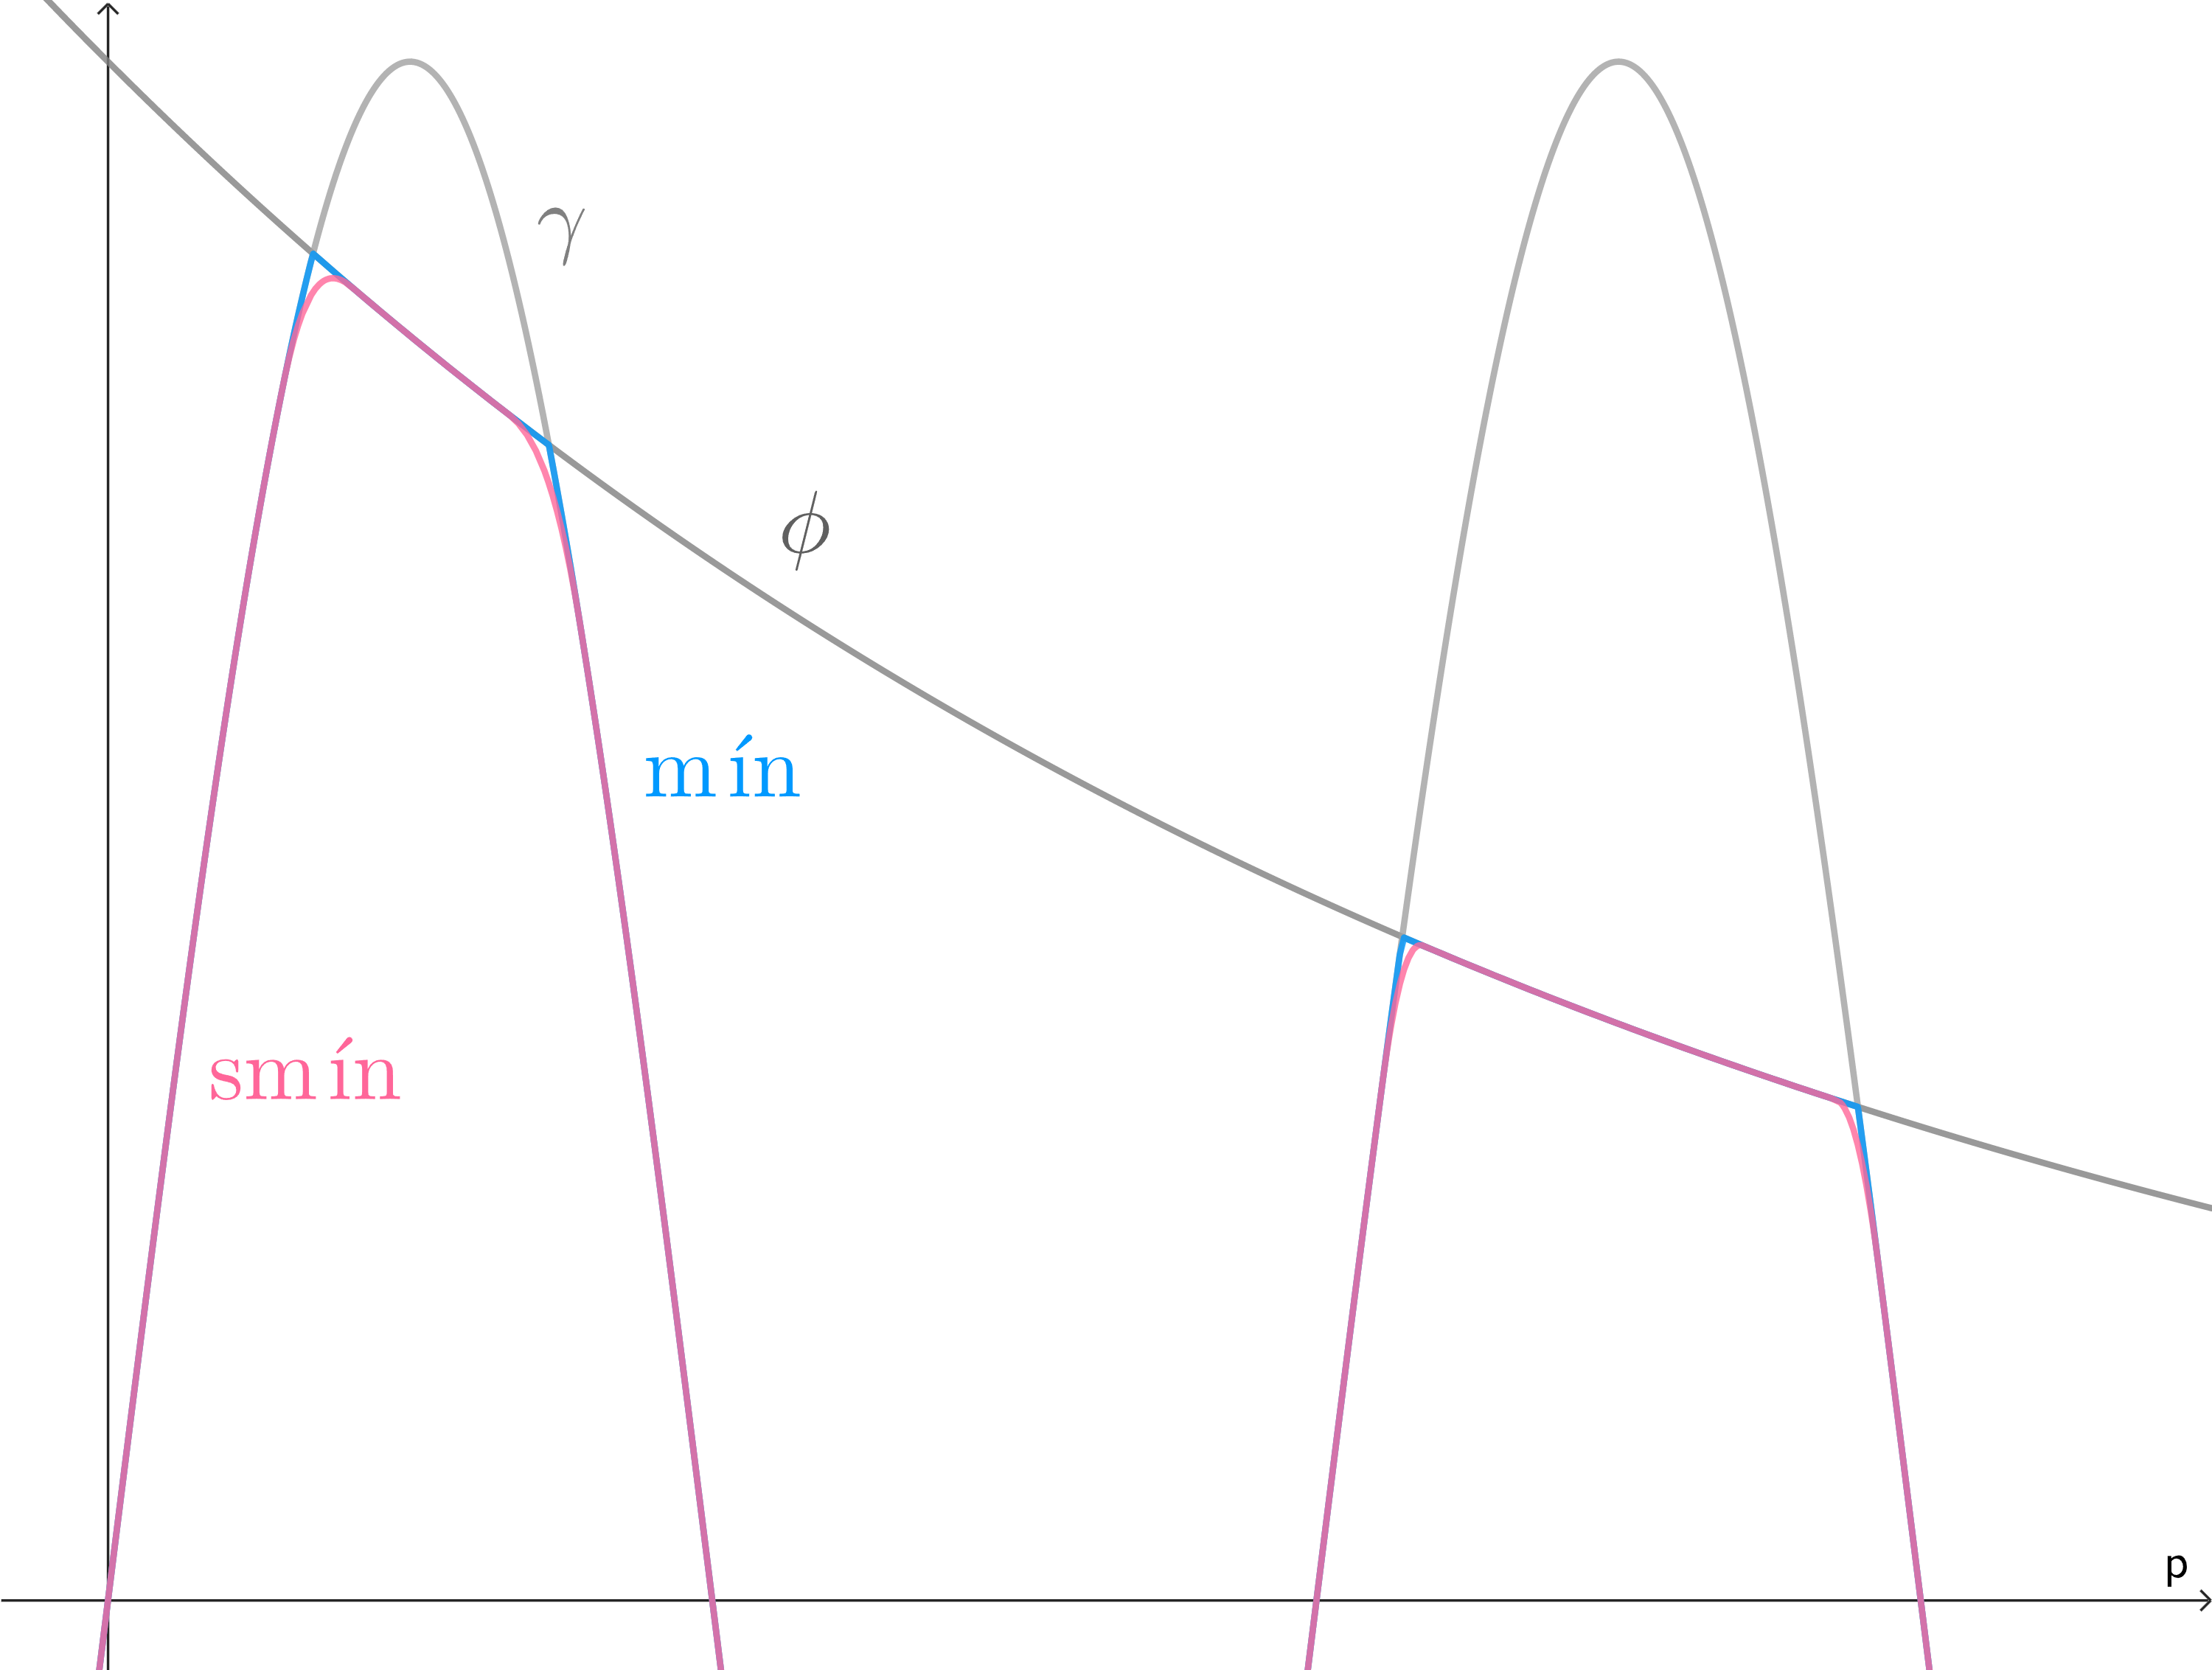
\includegraphics[width=0.95\textwidth]{Plantilla-TFG-master/img/smin_3.png}
        \caption{$k=0.1,\ n=2$}
     \end{minipage}
     \begin{minipage}[c]{0.49\linewidth}
        \centering
        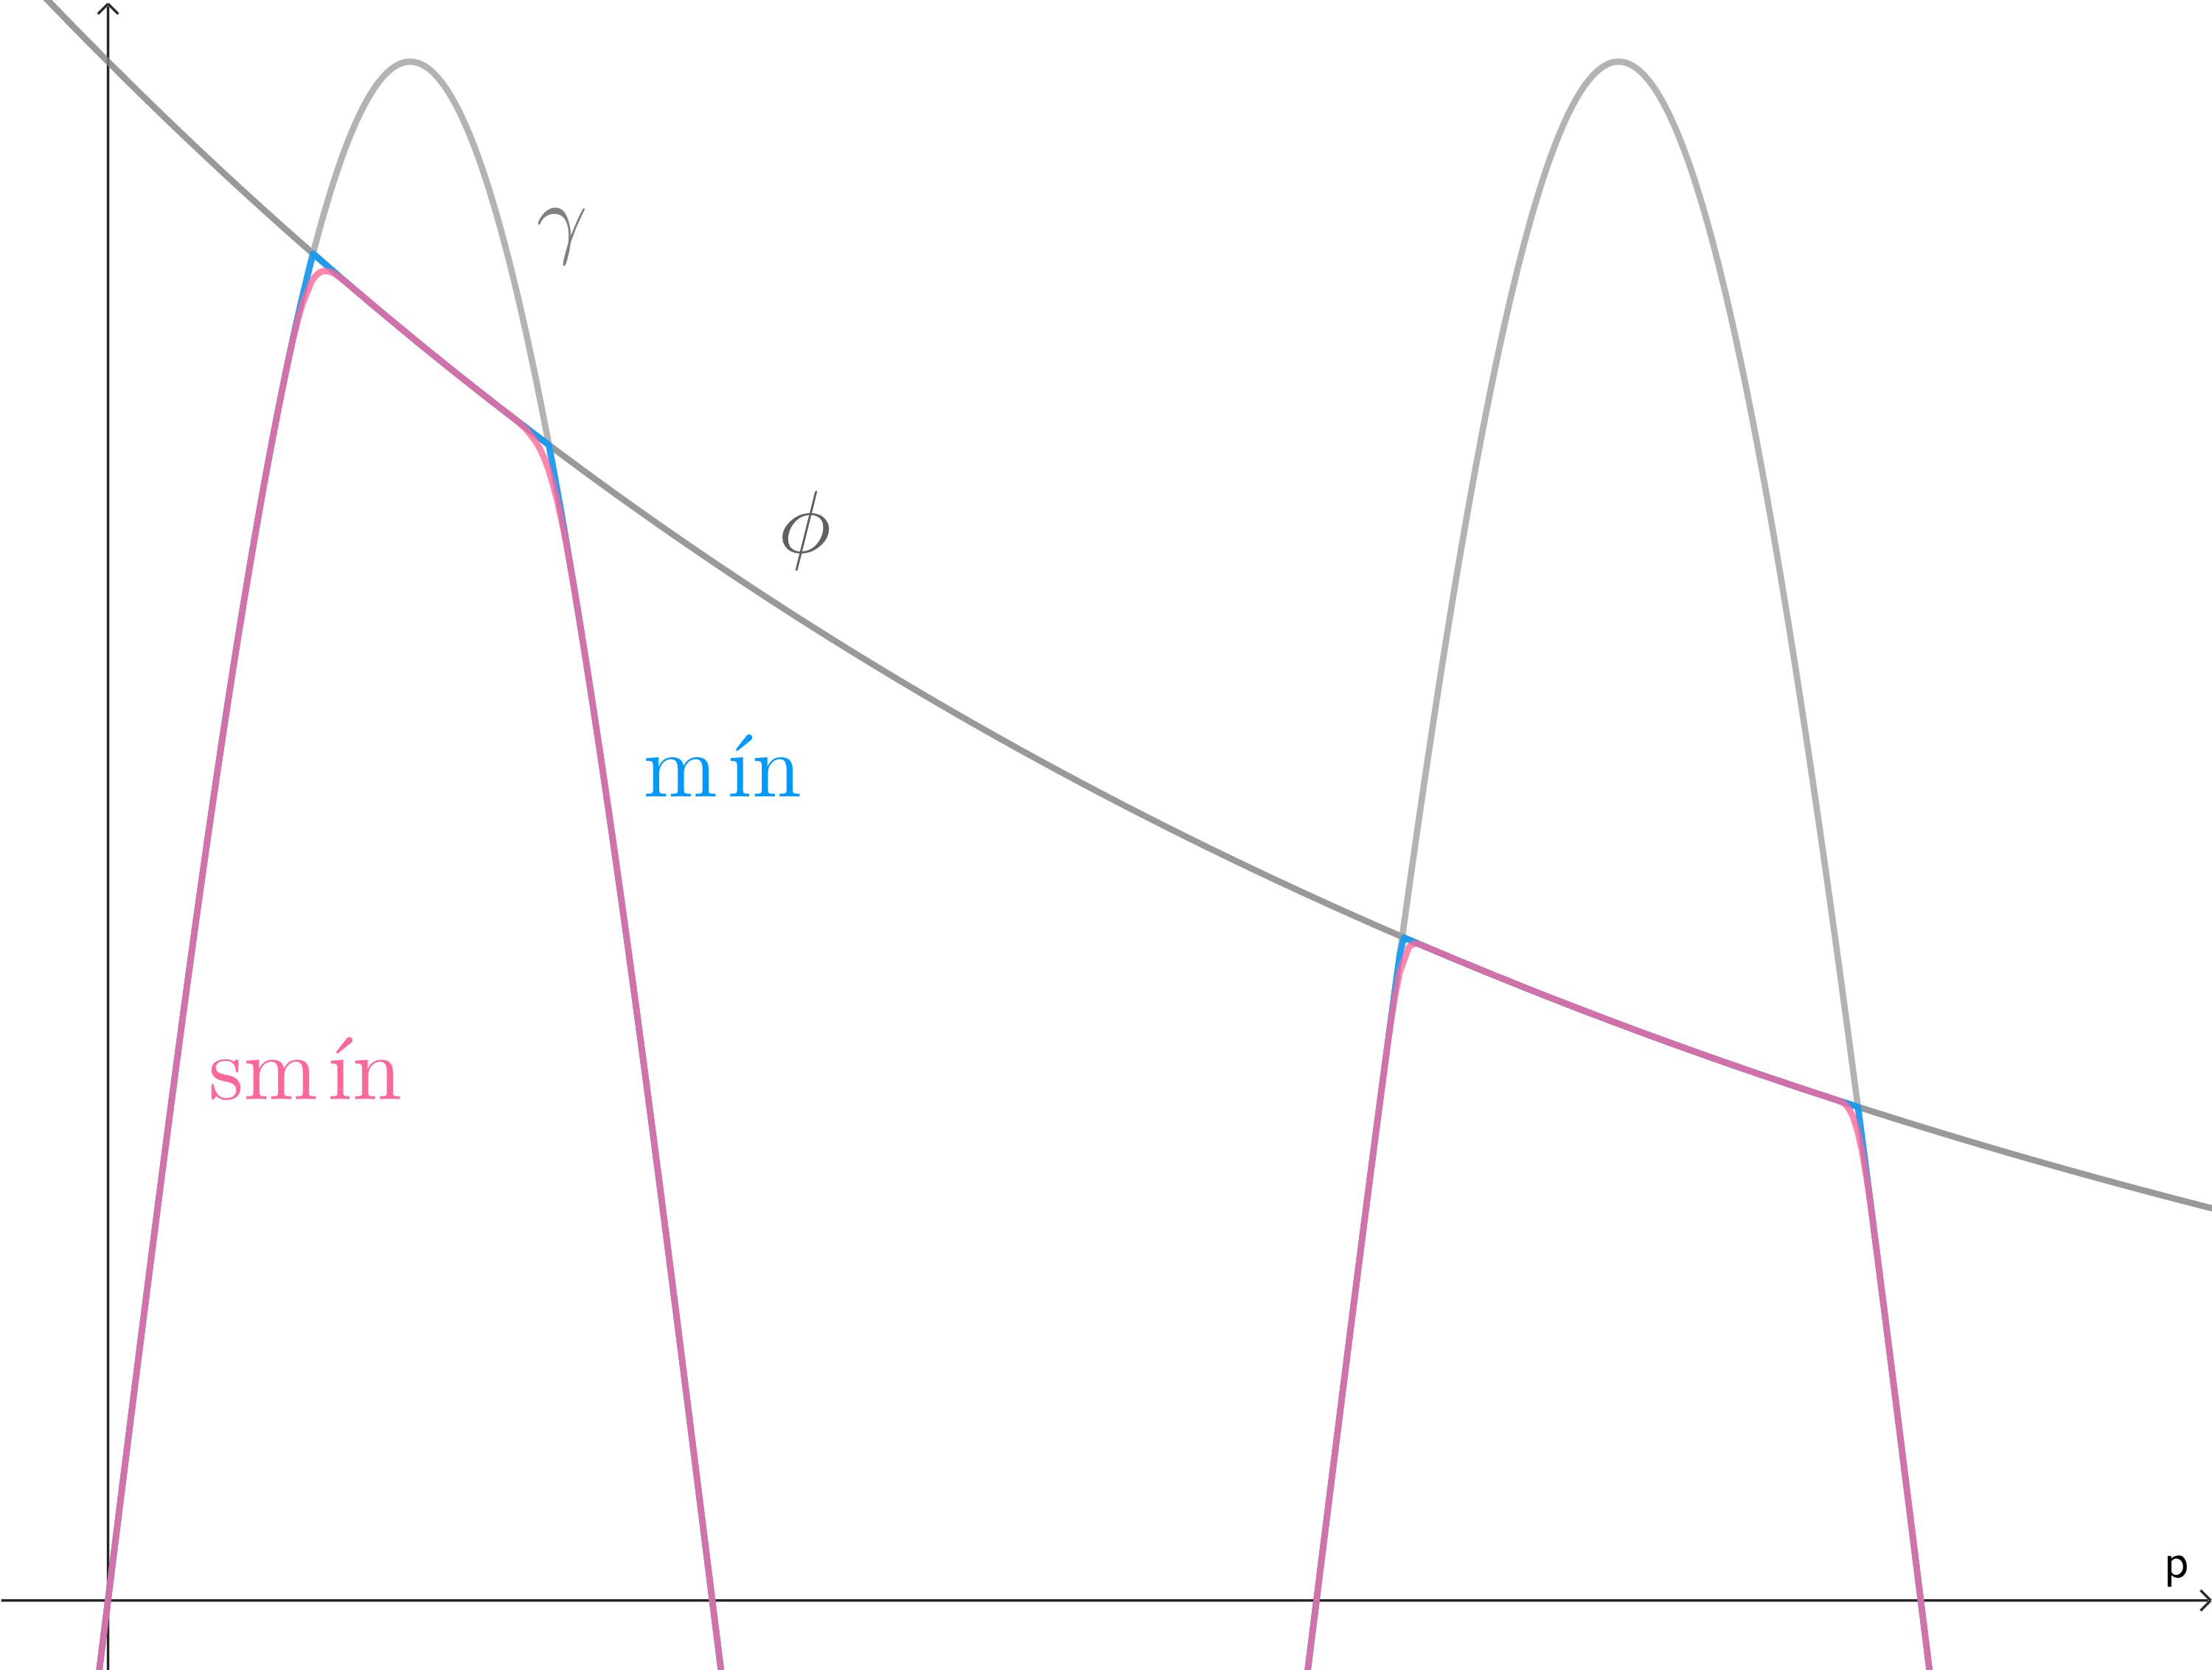
\includegraphics[width=0.95\textwidth]{Plantilla-TFG-master/img/smin_4.png}
        \caption{$k=0.1,\ n=3$}
     \end{minipage}
     \caption{Resultado final de $smin(p,k)$ }
     \label{fig:smooth2}
\end{figure}

Finalmente, para obtener una versión suavizada del máximo, es fácil comprobar que 
\begin{equation*}
    \smax(\phi,\gamma,k) =  - \smin(-\phi,-\gamma,k)
\end{equation*}

Recogemos los resultados obtenidos a continuación.



% Por tanto, dadas $\phi$ y $\gamma$, queremos obtener una versión suavizada de $\Min(\phi,\gamma)$ usando interpolación lineal, que llamaremos $\smin$ y tendrá la forma
% \begin{align*}
%           \smin\colon \R^3 &\to \R^3.\\
%           p &\mapsto h(p)\cdot \phi(p) + (1-h(p))\gamma(p) \text{, donde } h \colon \R^3 \to [0,1].
%     \end{align*}


% Pasamos a buscar $h$. Solo queremos modificar la función en los entornos de los puntos en los que intersecan $\phi$ y $\gamma$, de forma que para el resto de puntos debería ser $h=\{0,1\}$. Los puntos de intersección vienen dados como las soluciones de $m(p)=\gamma(p) - \phi(p)$. Podemos además acotar $m(p)$ en el intervalo $[0,1]$ usando $\Min$ y $\Max$, obteniendo un candidato a valor de $h(p)$:
% \begin{equation}
%     \Min\left(\Max\left(\phi(p)-\gamma(p),0\right),1\right) = \Min\left(\Max\left(m(p),0\right),1\right) \in [0,1]
% \end{equation}

% Sin embargo, podemos ver que la interpolación comienza justo en la intersección, mientras que nos gustaría que esto ocurriese antes. Modificamos la expresión anterior para hacer que la intersección sea el punto medio de la interpolación ($h=0.5$):
% \begin{equation}
%    \Min\left(\Max\left(m(p) + \frac{1}{2},0\right),1\right)
% \end{equation}

% Podemos ver los resultados de esta primera aproximación en la \autoref{fig:smooth1}.

% \begin{figure}[!h]
%      \begin{minipage}[c]{0.49\linewidth}
%         \centering
%         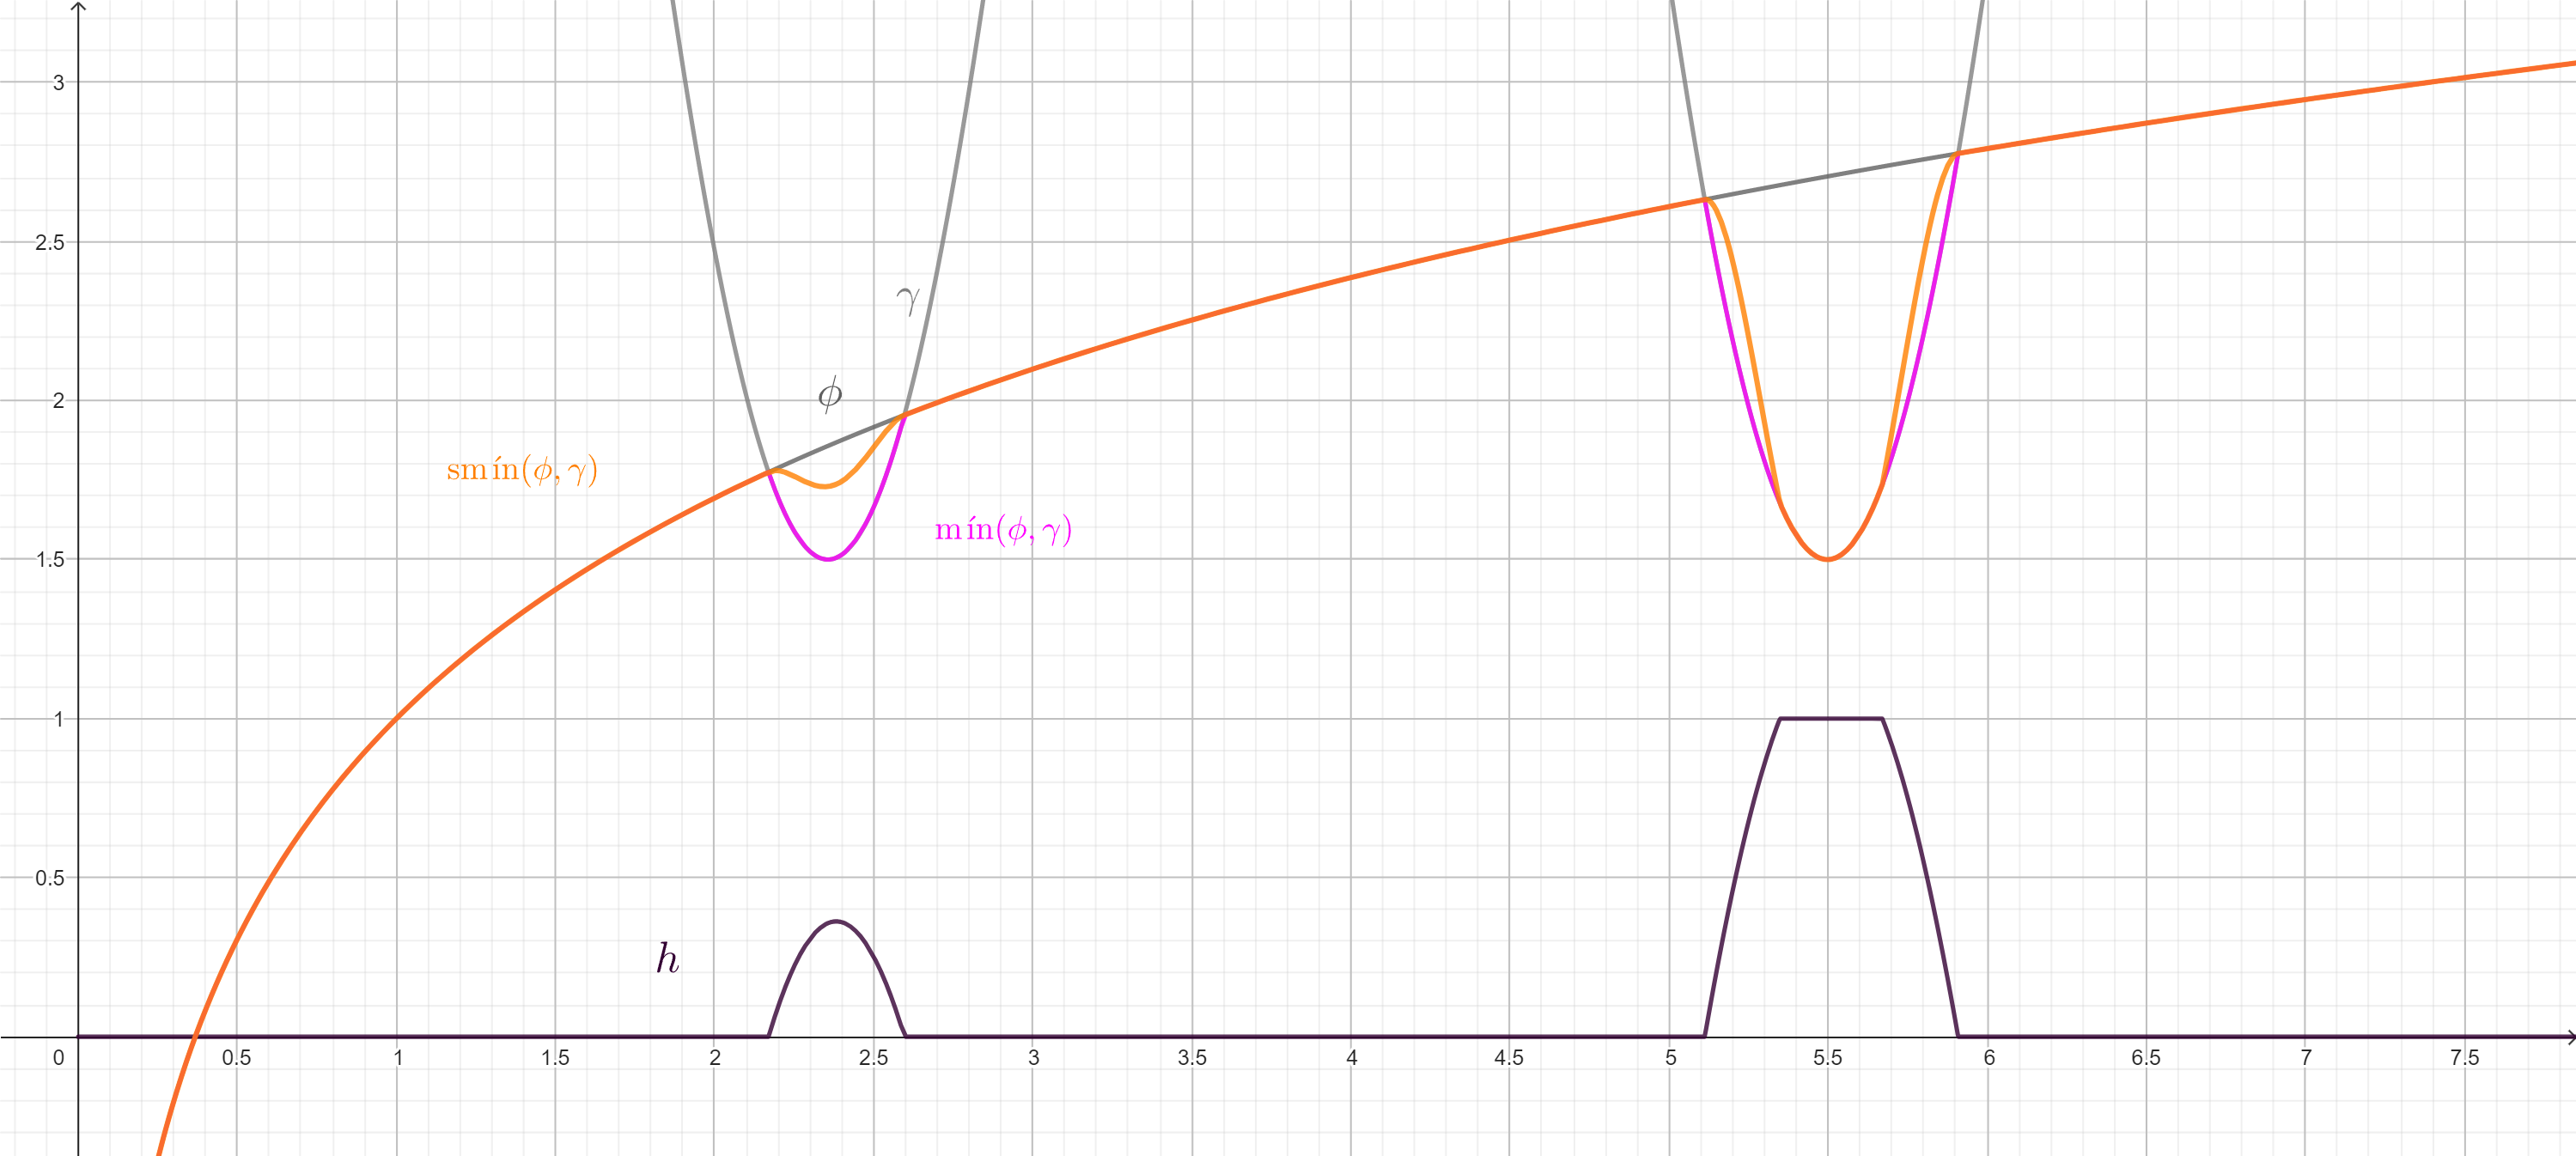
\includegraphics[width=0.95\textwidth]{Plantilla-TFG-master/img/smoothV1_a.png}
%         \caption{$h(p)=0$ en la intersección}
%      \end{minipage}
%      \begin{minipage}[c]{0.49\linewidth}
%         \centering
%         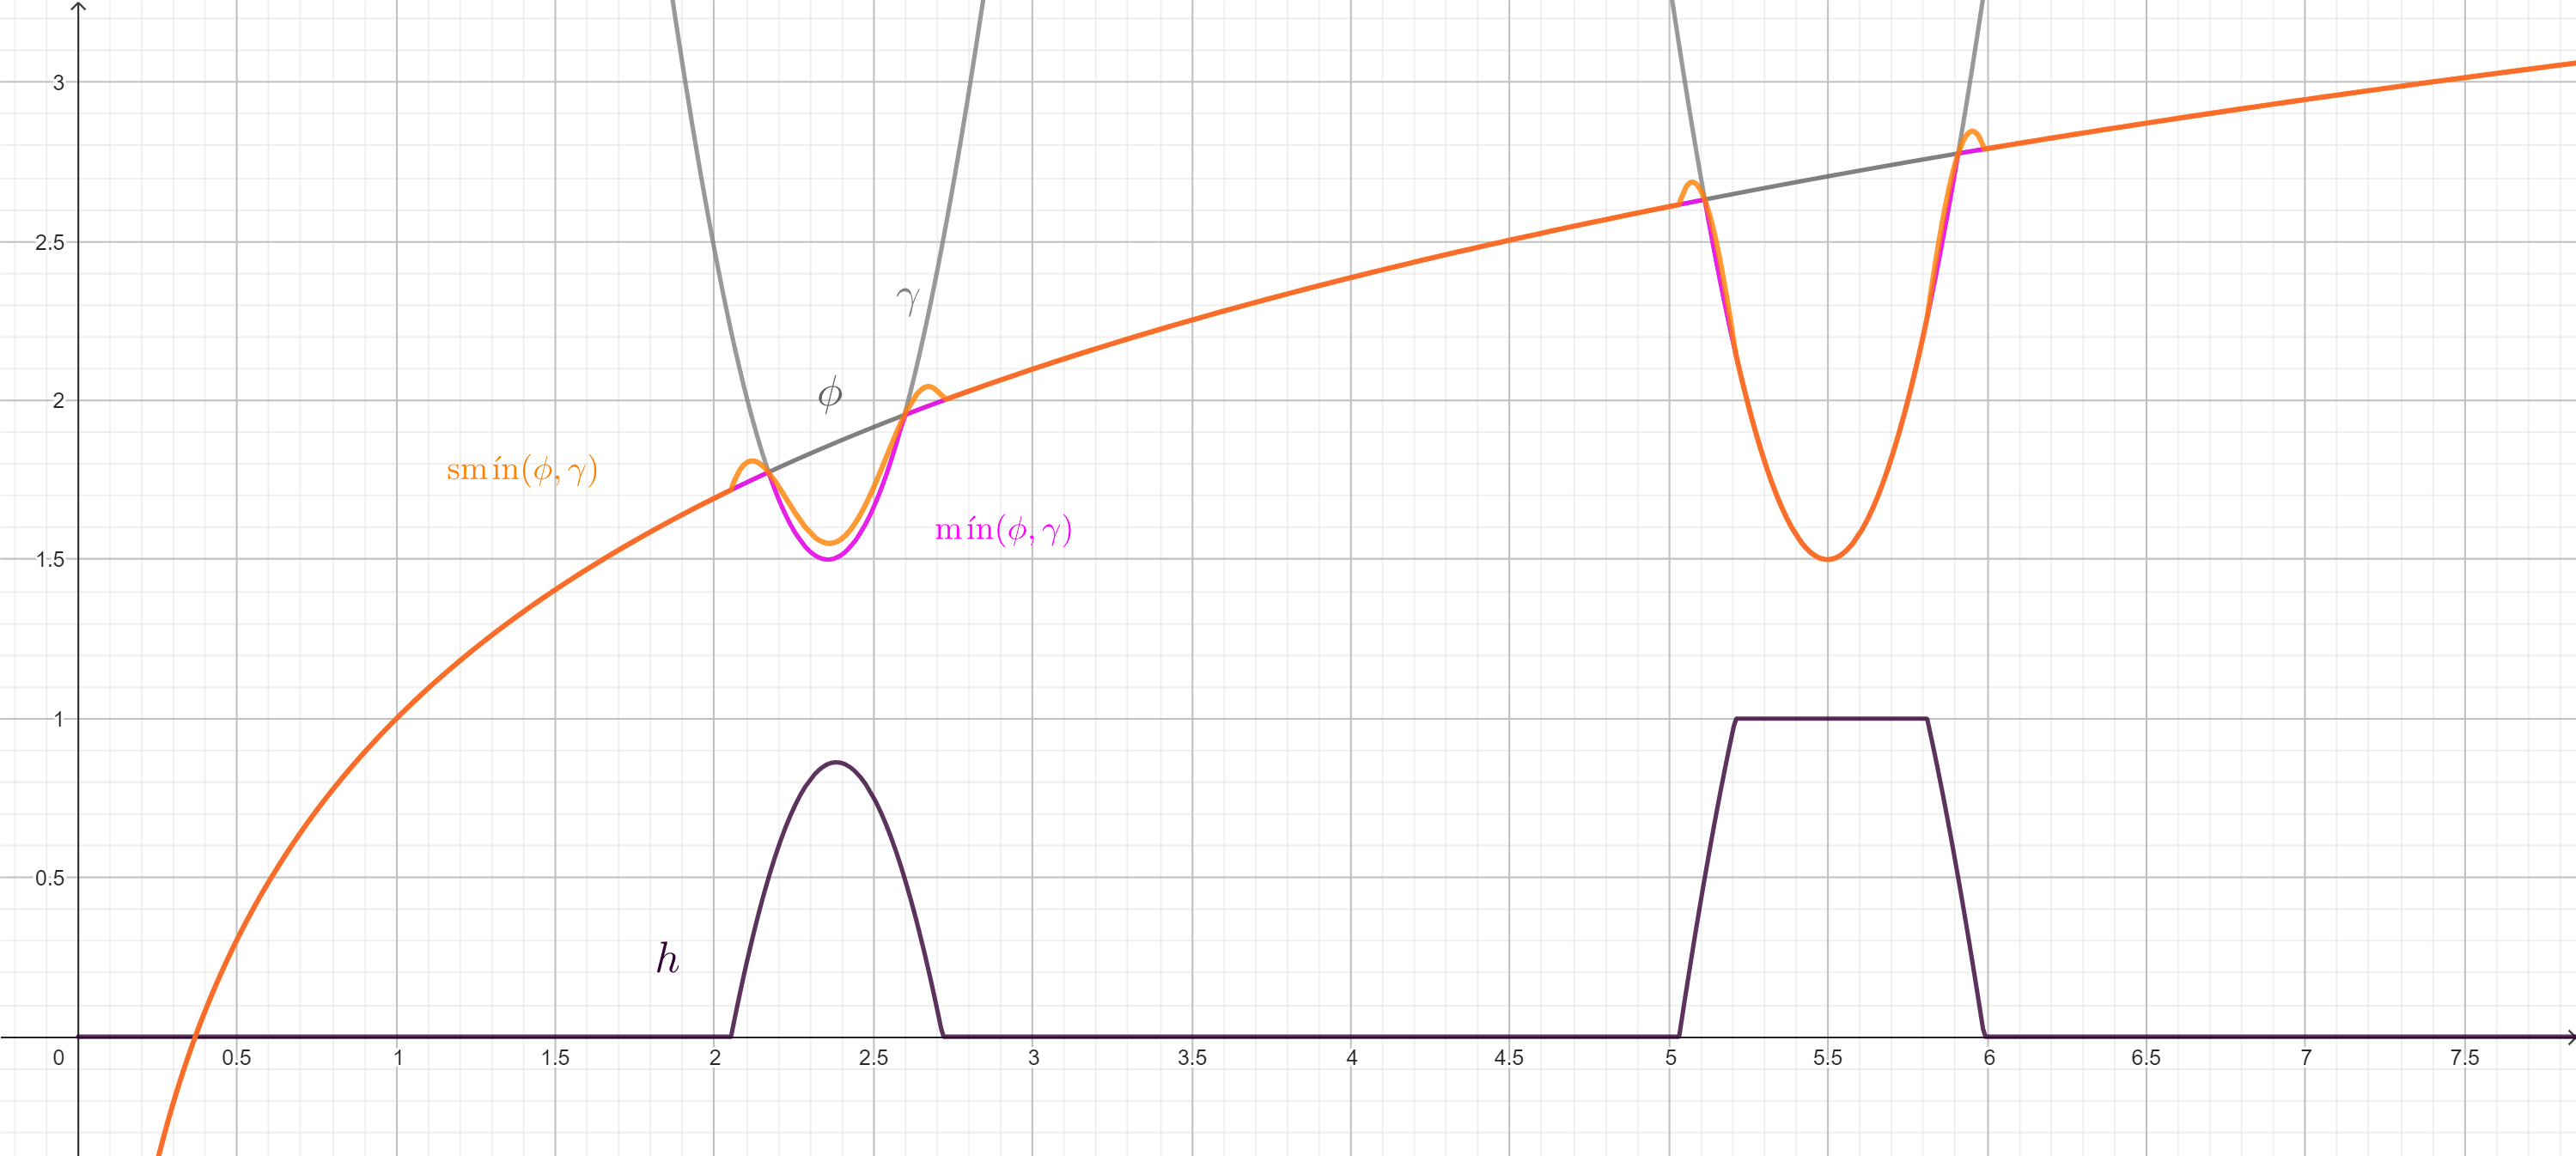
\includegraphics[width=0.95\textwidth]{Plantilla-TFG-master/img/smoothV1_b.png}
%         \caption{$h(p)=0.5$ en la intersección}
%      \end{minipage}
%      \caption{Primera aproximación de la obtención de $h(p)$}
%      \label{fig:smooth1}
% \end{figure}

% Observamos que ahora tenemos un nuevo problema

\begin{definicion}[Operaciones Booleanas Suavizadas]
    Sean $A$ y $B$ isosuperficies generadas por $\phi$ y $\gamma$ respectivamente. Definimos los SDF para las operaciones suavizadas como sigue.
    \begin{itemize}
        \item \textbf{Unión suavizada: } $\sdf_{unionS}(p) = \Min(\phi(p),\gamma(p)) - \frac{\Max\left( k - |\phi(p) - \gamma(p)|, 0\right)^n}{2n\cdot k^{n-1}}$,
        \item \textbf{Intersección suavizada: } $\sdf_{interS}(p) = -\Min(-\phi(p),-\gamma(p)) + \frac{\Max\left( k - |\phi(p) - \gamma(p)|, 0\right)^n}{2n\cdot k^{n-1}}$,
        \item \textbf{Diferencia suavizada: } $\sdf_{difS}(p) = -\Min(-\phi(p),\gamma(p)) + \frac{\Max\left( k - |\phi(p) + \gamma(p)|, 0\right)^n}{2n\cdot k^{n-1}}$,
    \end{itemize}

    donde $k\in \R^+_0$ es un coeficiente del suavizado.        
\end{definicion}

Observamos que los operadores definidos en la \autoref{p:boolean} no son más que un caso particular de estos últimos cuando $k= 0$.\newline


Pasamos ahora a estudiar otro tipo de operaciones, que nos resultarán útiles para generar nuevas formas a partir de un único SDF. Todas ellas se basarán en, dada $\phi$, aplicar una transformación $t:\R^3\to \R^3$ a cada punto de la isosuperficie $S_{\phi}$ para obtener una nueva $S_{\gamma}$. Si queremos saber si un punto $q\in\R^3$ está en $S_{\gamma}$, tenemos que comprobar si su preimagen por la transformación pertenece a $S_{\phi}$. Por tanto, bastará evaluar el SDF original en $t^{-1}(p)$, obteniendo que
\begin{equation*}
    \gamma(p) = \phi(t^{-1}(p))
\end{equation*}

Esto funciona bien para transformaciones como las traslaciones o rotaciones, ya que mantienen las distancias. Sin embargo, este no es el caso del escalado, ya que si tomamos $l(p) = sp$ con $s\in \R^+_0$:
\begin{equation*}
    \Vert p-p'\Vert = l(d) \implies  \Vert l(p)-l(p')\Vert = \Vert sp-sp'\Vert = s\Vert p-p'\Vert = s\cdot d,\  \text{ donde } p,p' \in A
\end{equation*}

Como las distancias se escalan, deberemos hacer lo propio con el nuevo SDF, aplicándole el mismo factor de escalado $s$ como muestra la \autoref{d:afines}.

\begin{definicion}[Operaciones afines]\label{d:afines}
    Sea $A$ una isosuperficie. Definimos los SDF para las siguientes operaciones.
    \begin{itemize}
        \item \textbf{Traslación de vector $\boldsymbol{v}$: } $\sdf_{traslacion}(p) = \sdf_{A}(p - v)$,
        \item \textbf{Escalado uniforme de dimensiones $\boldsymbol{s}$: } $\sdf_{escalado}(p) = \sdf_{A}(p/s)\cdot s$,
        \item \textbf{Rotaciones de ángulo $\boldsymbol{\alpha}$ sobre los ejes $\boldsymbol{x,y,z}$: }
        \begin{align*}
            \sdf_{rotX}(p) &= \sdf_{A}(R_x^{-1}(\alpha)\cdot p^t),\ R_x(\alpha) = 
            \begin{pmatrix}
                1&0&0\\
                0&\cos(\alpha) & -\sin(\alpha) \\
                0&\sin(\alpha) & \cos(\alpha) 
                \end{pmatrix},\\[10pt] 
            \sdf_{rotY}(p) &= \sdf_{A}(R_y^{-1}(\alpha)\cdot p^t),\ R_y(\alpha) = \begin{pmatrix}
            \cos(\alpha) &0& \sin(\alpha)\\
            0&1&0\\
            -\sin(\alpha) &0& \cos(\alpha) 
            \end{pmatrix},\\[10pt]
            \sdf_{rotZ}(p) &= \sdf_{A}(R_z^{-1}(\alpha)\cdot p^t),\ R_z(\alpha) = \begin{pmatrix}
            \cos(\alpha) & -\sin(\alpha) & 0\\
            \sin(\alpha) & \cos(\alpha) & 0\\
            0&0&1
            \end{pmatrix}.
        \end{align*}
        
    \end{itemize}
\end{definicion}

Siguiendo el mismo razonamiento, podemos definir operaciones que modifiquen la geometría de la superficie.
\begin{definicion}[Operaciones Deformantes]
    Sea $A$ una isosuperficie. Definimos los SDF para las siguientes operaciones.
    \begin{itemize}
        
        \item \textbf{Torsión: } $\sdf_{torsion}(p) = \sdf_{A}(p')$, con $p' = R_z(ky)\cdot (x,z,y)^t$,
        \item \textbf{Plegado: } $\sdf_{plegado} =\sdf_{A}(p')$, con $p' = R_z(kx)\cdot p^t$,
        \item \textbf{Redondeo: } $\sdf_{redondeo}(p) = \sdf_{A}(p) - k$,
        \item \textbf{Desplazamiento: } $\sdf_{desplazamiento}(p) = \sdf_{A}(\delta(p))$.
    \end{itemize}

    donde
    \begin{itemize}
        \item $k\in \R^+_0$ es un coeficiente de deformación,
        \item $\delta\colon \R^3\to \R^3$ es un patrón de desplazamiento,
        \item $R_z(\alpha)\in \mathcal{M}_3(\R)$ es la matriz de rotación de ángulo $\alpha$ sobre el eje $z$ dada en la \autoref{d:afines}.
    \end{itemize}
\end{definicion}

Introducimos por último operaciones que permiten generar copias de otras superficies.
\begin{definicion}[Operadores de Posicionamiento]\label{d:posicionamiento}
    Sea $A$ una isosuperficie. Definimos los SDF para las siguientes operaciones.
    \begin{itemize}
        \item \textbf{Simetrías sobre los ejes $\boldsymbol{x,y,z}$:}
        \begin{gather*}
            \sdf_{simX}(p) = \sdf_{A}(\vert x\vert, y, z),\quad \sdf_{simY}(p) = \sdf_{A}(x, \vert y\vert,  z),\\[5pt] \sdf_{simZ}(p) = \sdf_{A}(x,y,\vert z\vert),
        \end{gather*}
        \item \textbf{Simetrías sobre los planos $\boldsymbol{xy,xz,yz}$:}
        \begin{gather*}
            \sdf_{simXY}(p) = \sdf_{A}(\vert x\vert, \vert y\vert, z),\quad \sdf_{simXZ}(p) = \sdf_{A}(\vert x\vert, y,  \vert z\vert),\\[5pt]\sdf_{simYZ}(p) = \sdf_{A}(x,\vert y\vert ,\vert z\vert),
        \end{gather*}
        \item \textbf{Repetición $\boldsymbol{l\in \N^3}$ veces en los ejes $\boldsymbol{x,y,z}$ con separación $\boldsymbol{s\in\R}$:} 
        \begin{equation*}
            \sdf_{rep}(p) = \sdf_{A}(p - s\cdot c\left(r(p/s)), -l, l\right),
        \end{equation*}
        \item \textbf{Repetición infinita:}
        \begin{equation*}
            \sdf_{repInf}(p) = \sdf_{A}\left((p+\frac{l}{2}\mod l )- \frac{l},{2}\right)
        \end{equation*}
    \end{itemize}
    donde:
    \begin{itemize}
        \item $c\colon \R\times\R\times\R\to \R,\ c(x,a,b) = \Min(\Max(x, a), b)$ acota $x$ en $[a,b]$,
        \item $r\colon \R^3 \to \R^3$ redondea las componentes de un vector a sus enteros más cercanos.
    \end{itemize}
\end{definicion}
\begin{observacion}
    Hay casos en los que los SDF definidos en la \autoref{d:posicionamiento} podrían no ser exactos, al igual que ocurría con la intersección y la diferencia en la \autoref{p:boolean}:
    \begin{enumerate}
        \item Para las simetrías, cuando el objeto interseca el plano de simetría,
        \item Para las repeticiones, cuando las dimensiones del objeto sean mayores o iguales a $l/2$.
    \end{enumerate}
\end{observacion}

A la vista de todas esta operaciones a nuestra disposición, es evidente el potencial que tienen los SDF, tanto en la generación y modificación de figuras como en su eficiencia, ya que podemos visualizar miles de objetos al precio de uno utilizando las simetrías o repeticiones.

\section{Raymarching y Spheretracing}
Una vez definida la escena necesitamos un método para visualizarla. Utilizaremos la técnica de \textit{raymarcing}. Para ello deberemos elegir un punto donde estará el observador. A partir de él se trazarán rayos hacia cada uno de los puntos de un plano imaginario que llamaremos plano de visión, de forma que cada punto de este plano corresponde a un pixel de la imagen resultante. Si el rayo interseca con $S_\phi$ significa que ese pixel corresponde a un punto de $S_\phi$ y será coloreado como tal.\newline

Para comprobar esta intersección utilizamos un método iterativo: a partir de la posición del observador, en cada iteración avanzamos en la dirección del rayo una distancia fija $\delta$. Evaluamos entonces nuestro SDF en la posición actual. Si este valor es muy cercano a 0 significará que estamos en la isosuperficie. De lo contrario, repetiremos el proceso hasta encontrar la intersección o superar el número máximo de iteraciones, en cuyo caso concluiremos que no hay intersección.\newline

TODO: diagrama

Sin embargo podemos mejorar esta técnica, ya que cuanto más alejados estén los puntos de $S_\phi$ del observador, mayor es el número de iteraciones necesarias para encontrar la intersección. Esto es debido a que si no queremos perder ninguna intersección, el valor de incremento $\delta$ deberá de ser pequeño. La solución a este problema es el uso de \textit{spheretracing}. Su funcionamiento es similar al \textit{raymarching}, con la diferencia de que el incremento en la posición del rayo no es fija, sino que es la máxima que podemos tomar asegurándonos de no perder información en cada iteración. Esta distancia será entonces la distancia mínima del punto actual del rayo a $S_\phi$, que no es más que evaluar $\phi$ en dicho punto.\newline

TODO: diagrama de pérdida de intersección

El algoritmo sería por tanto el descrito en \autoref{a:spheretracing}. 
\SetKwComment{Comment}{/* }{ */}
\begin{algorithm}[hbt!]\label{a:spheretracing}
    \caption{Spheretracing}\label{alg:spheretracing}
    \KwData{origen $p$, dirección $v$}
    $\text{incremento} \gets 0$\;
    $\text{distanciaTotal} \gets 0$\;
    
    \For{i \in MAX\_ITERACIONES} {
        rayo \gets p + \text{distanciaTotal}\cdot v\;
        
        distanciaActual \gets \phi(\text{rayo})\;
        
        \If{distanciaActual < \varepsilon}{
           \Return{DibujarSuperficie(rayo)};
        }

        distanciaTotal \mathrel{{+}{=}} distanciaActual\;

        \If{distanciaTotal > MAX\_DISTANCIA}{
            \Return{DibujarFondo()};
        }
    }
\end{algorithm}

\section{Iluminación}
Ya sabemos qué píxeles pertenecen a la superficie, pero no de qué color deben dibujarse. Para ello utilizaremos el modelo de reflexión de Phong. En él trabajaremos con los siguientes parámetros:
\begin{itemize}
  \item Luz ambiente $i_a$: vector RGB suma de las contribuciones de todas las fuentes de luz de la escena. Contiene un valor por defecto que será el color del fondo.
  \item Lista de fuentes de luz $(l_1, \dots, l_m, \dots, l_n)$.
  \item Materiales asignados a cada objeto definidos por las constantes:
      \begin{itemize}
          \item Reflexión especular $k_s$: modela cómo se refleja la luz en objetos brillantes. Depende tanto de la posición de las fuentes de luz como de la del observador.
          \item Reflexión difusa $k_d$: modela cómo se refleja la luz en objetos mates. Depende de la posición de las fuentes de luz, pero no de la posición del observador.
          \item Reflexión ambiental $k_a$: representa la proporción de luz del ambiente que refleja el objeto.
          \item Coeficiente de brillo $\alpha$: valor real positivo que permite variar el tamaño de las zonas brillantes (a mayor valor, menor tamaño y más pulida o especular).
      \end{itemize}
  
  \item Los vectores normalizados definidos para cada punto de la superficie $p$:
        \begin{itemize}
          \item $L_m$: vector director desde $p$ a cada fuente de luz $l_m$.
          \item $N$ vector normal a la superficie en $p$.
          \item $R_m$ dirección del rayo de luz reflejado especularmente desde la fuente $l_m$ en el punto $p$.
          \item $V$: dirección de $p$ a la posición del observador.
        \end{itemize}
\end{itemize}

TODO: diagrama vectores

Con estas variables, el color en $p$ vendrá dado por la fórmula:
\begin{equation*}
  I_p = k_a i_a + \sum_{m=0}^{n} \left(k_d\left(L_m\cdot N\right) + k_s\left(R_m\cdot V\right)^{\alpha} \right)
\end{equation*}

De los vectores anteriores, $L_m$ y $V$ se calculan trivialmente, y $R_m$ se puede obtener como
\begin{equation*}
  R_m = 2(L_m\cdot N)N - L_m
\end{equation*}

Veamos como obtener $N$.

\subsection{Cálculo del vector normal}
\begin{definicion}
  El \textbf{gradiente} de una función implícita $\phi\colon \R^3\to\R$ es $\nabla\phi = \left(\frac{\partial \phi}{\partial x}, \frac{\partial \phi}{\partial y}, \frac{\partial \phi}{\partial z}\right)$.
\end{definicion}

\begin{proposicion}\label{p:gradient_perp}
  $\nabla\phi$ es perpendicular a $S_\phi$.
\end{proposicion}

\begin{proof}
  Sea $s\in S_\phi$ arbitrario. Tomamos una curva parametrizada:
  \begin{align*}
    \alpha \colon [0,1] & \to S_\phi                             \\
    t                   & \mapsto \left(x(t), y(t), z(t) \right)
  \end{align*}

  cumpliendo $\alpha(t_0)=s$. Veamos que $\nabla\phi(s) \perp \alpha$:

  \begin{align*}
    \alpha(t)\subset S_\phi & \implies \phi(\alpha(t))=0\\
                            & \implies \nabla\phi(\alpha(t)) = \frac{\partial{F}}{\partial{x}}\frac{dx}{dt} + \frac{\partial{F}}{\partial{y}}\frac{dy}{dt} + \frac{\partial{F}}{\partial{z}}\frac{dz}{dt} = 0 \\
                            & \implies \langle \nabla\phi(x,y,z), \alpha'(t)\rangle = 0 \implies \langle \nabla\phi(x,y,z), \alpha'(t_0)\rangle = 0
  \end{align*}

    Por tanto, $\nabla\phi(s)$ es perpendicular al vector tangente de $\alpha$ en $s$, que a su vez está contenida en el plano tangente de $S_\phi$ en $s$. Por tanto $\nabla\phi(s) \perp S_\phi$.
\end{proof}

Hemos visto que calcular $N$ equivale a calcular $\nabla\phi$. Sin embargo, dado que la superficie viene dada por un SDF que podría ser no derivable, no podemos hacerlo de forma analítica. De ser derivable, podría ser una buena opción calcular el gradiente una única vez al momento de definir la $\phi$, tras lo cual para obtener $N$ solo habría que realizar evaluaciones de dicho gradiente. Sin embargo, por su sencillez y popularidad, nos decantaremos por un método numérico que únicamente hará uso de evaluaciones de $\phi$.

\begin{definicion}
  Dada $\phi:\R^3\to \R$ diferenciable, $p = (x,y,z)$, $v\in \R^3$, definimos la \textbf{derivada direccional} en $p$ con dirección $v$ a:
  \begin{equation*}
    \nabla_v f(p) = \nabla f(p) \cdot v = \frac{\partial{f}(p)}{\partial{x}}v_x + \frac{\partial{f}(p)}{\partial{y}}v_y + \frac{\partial{f}(p)}{\partial{z}}v_z
  \end{equation*}
\end{definicion}

Para el cálculo de cada parcial de $f$ podemos utilizar la definición de derivada. Por ejemplo, para la primera componente:
\begin{equation*}
  \frac{\partial{f}(p)}{\partial{x}} v_x = \lim_{h\to 0}\frac{f(p + (h,0,0)) - f(p)}{h} v_x
\end{equation*}

Procedemos a calcular $N$ aplicaremos el \textbf{método del tetraedro}, el cual se basa en evaluar $\phi$ en la dirección de los vértices de un tetraedro:

\begin{equation*}
    k_0 = (1,-1,-1)\quad k_1 = (-1,-1,1)\quad k_2=(-1,1,-1)\quad k_3=(1,1,1)
\end{equation*}

\begin{proposicion}[Método del tetraedro]
  Dado $p\in S_\phi$, su vector normal $N$ se obtiene normalizando el vector
  \begin{equation*}
    \hat{N} = \sum_{i=0}^3 k_i\cdot f(p + hk_i)
  \end{equation*}
\end{proposicion}

\begin{proof}
  Por la proposición \autoref{p:gradient_perp}, basta comprobar que $\hat{N}$ es colineal a $\nabla \phi(p)$.

  \begin{align*}
    \hat{N} & = \sum_{i=0}^3 k_i\cdot f(p + hk_i) = \sum_{i=0}^3 k_i\cdot f(p + hk_i) + k_i\cdot f(p) = \sum_{i=0}^3 k_i\cdot f(p+hk_i - f(p)) = \sum_{i=0}^3 k_i \nabla_{k_i}f(x)\\
    &= \sum_{i=0}^3 k_i \cdot \left( k_i \cdot \nabla f(p)\right) = \sum_{i=0}^3 (k_i\cdot k_i) \nabla f(p) = \sum_{i=0}^3 \nabla f(p) = 4\nabla f(p)
  \end{align*}

  donde hemos usado que $\sum_{i=0}^3 k_i = (0,0,0)$, $\sum_{i=0}^3 k_i\cdot k_i = (1,1,1)$, y que el producto escalar es un operador lineal.
\end{proof}

\section{Aproximación de implícitas}
Empezábamos el capítulo diciendo que una de las representaciones más comunes de superficies es a través de implícitas, pero hasta ahora nos hemos centrado en estudiar un tipo particular de este tipo de ecuaciones. Si intentásemos aplicar los algoritmos anteriores a una función implícita cualquiera, observaríamos que el resultado tiene ciertos defectos, tales como deformaciones, o incluso no se visualiza. Vamos a introducir una técnica que dada una función implícita $\phi$, nos permitirá obtener un SDF aproximado de $S_\phi$. Esto nos será útil cuando no conozcamos o no podamos calcular explícitamente el SDF de una superficie pero sí su representación implícita.

\begin{proposicion}
    Sea $\phi\colon \R^3\to\R$ una función implícita cualquiera y $p\in\R^3$. Entonces: 
    \begin{equation*}    
        \sdf_{S_\phi}(p) \approx \frac{\vert \phi(p)\vert}{\vert \nabla\phi(p)\vert}
    \end{equation*}
\end{proposicion}
\begin{proof}
    Sea $q$ al punto de $S_\phi$ más cercano a $p$ y $v=\vec{pq} \perp S_\phi$ en $q$. Queremos calcular la distancia de $p$ a $S_\phi$, que es justamente $v$. Podemos calcular el desarrollo de Taylor de $\phi$ en $p$:
    \begin{equation*}
        \phi(p+v) = \phi(p) + \nabla(p)\cdot (p+v-p) + \mathcal{O}(\vert p+v-p\vert^2) \implies \phi(p+v) = \phi(p) + \nabla(p)\cdot v + \mathcal{O}(\vert v\vert^2)
    \end{equation*}

    Suponemos ahora que $p$ está cerca de $S_\phi$, esto es, $\vert v\vert < \varepsilon$. Como $\phi(p+v) = \phi(q)=0$, tenemos que:
    \begin{align*}
        0 &= \vert \phi(p+v)\vert \approx \vert \phi(p) + \nabla(p)\cdot v \vert \le \vert \phi(p)\vert - \vert \nabla(p)\cdot v \vert\\
         &\le \vert \phi(p)\vert - \vert \nabla(p)\vert \vert v \vert \implies \vert v\vert \le \frac{\vert \phi(p)\vert}{\vert \nabla(p)\vert}
    \end{align*}
    donde hemos usado la desigualdad triangular y las propiedades del producto escalar.
\end{proof}

Al igual que nos ocurría al calcular el vector normal, habrá ocasiones en las que el gradiente no pueda ser obtenido de forma analítica. Esta vez sin embargo no nos basta con conocer solo la dirección del gradiente, así que no podemos aplicar de nuevo el método del tetraedro. Usaremos un nuevo método en su lugar que usa la definición de derivada.

\begin{proposicion}[Método de las diferencias centrales]
    Sea $\phi\colon \R^3\to\R$. Entonces:
    \begin{align*}
        \frac{\partial\phi}{\partial x}(p) &\approx \frac{\phi(p+(h,0,0)) - \phi(p-(h,0,0))}{2h}\\[10pt]
        \frac{\partial\phi}{\partial y}(p) &\approx \frac{\phi(p+(0,h,0)) - \phi(p-(0,h,0))}{2h}\\[10pt]
        \frac{\partial\phi}{\partial z}(p) &\approx \frac{\phi(p+(0,0,h)) - \phi(p-(0,0,h))}{2h}
    \end{align*}
    
    donde $h\in\R^+$ es un valor arbitrariamente pequeño. 
\end{proposicion}

Para calcular el gradiente necesitaremos evaluar $\phi$ un total de seis veces, ya que hay que realizar dos evaluaciones por cada variable. Es por este motivo que 




